\documentclass[10pt]{beamer}
\usepackage{appendixnumberbeamer}
\usepackage[numbers,sort&compress]{natbib}
\usepackage{booktabs}
\usepackage[scale=2]{ccicons}
\usepackage{graphicx}
\usepackage{xspace}
\usepackage{media9}
\usepackage{tikz}
\usepackage{colortbl}
\usepackage{multirow}
\usepackage[portuguese]{babel}
\usepackage{subfigure}
\usepackage{comment}
\usepackage{wrapfig}
\usetheme[progressbar=frametitle]{metropolis}
\newcommand{\themename}{\textbf{\textsc{metropolis}}\xspace}
\bibliographystyle{rusnat}
\usetikzlibrary{arrows,positioning}
\definecolor{boxcolor}{HTML}{B9DCFF}
\tikzset{block/.style={draw, fill=boxcolor, minimum size=2em, text width =
         1.8cm, align = center, minimum height = 1.5cm},
         arrow/.style={->, red, text = black}}




\title{Modelos de Inteligência Computacional aplicados ao Sistema Epidemiológico}
\author{João Samuel Maciel de Sales}
\institute{Universidade Federal do Ceará}
\date{\today}
\titlegraphic{\hfill
\includegraphics[height=2cm]{figuras/logo.PNG}}

\begin{document}

\maketitle

\begin{frame}{SUMÁRIO}
    \setbeamertemplate{section in toc}[sections numbered]
    \tableofcontents[hideallsubsections]
\end{frame}

\section{Introdução}
\begin{frame}{Introdução}
    \begin{enumerate}

        \item Devido aos diversos desafios e adversidades na busca pela sobrevivência, a sociedade humana evoluiu ao longo dos anos;

              \vspace{0.5cm}


        \item Entretanto, nenhum outro motivo traz tanto medo à sociedade quanto as doenças, principalmente as infecciosas que foram responsáveis por enorme sofrimento e morte ao longo da história \cite{schecter2021};

              \vspace{0.5cm}


        \item Por isso, será apresentado um breve entendimento sobre as doenças infecciosas virais em especial a doença do novo coronavírus.

    \end{enumerate}
\end{frame}

\begin{frame}{Classificação de doenças infecciosas virais}



    De acordo com a Organização Mundial da Saúde (OMS), estas doenças podem ser classificadas da seguinte forma:

    \vspace{0.5cm}

    %\pause 

    \begin{enumerate}

        \item Surto;

              %\pause    
              \vspace{0.5cm}


        \item Endemia;

              %\pause
              \vspace{0.5cm}


        \item Epidemia;

              %\pause
              \vspace{0.5cm}


        \item Pandemia.

    \end{enumerate}
\end{frame}

\begin{frame}{Tipos de transmissão de doenças infecciosas virais}

    Modos de transmissão

    \vspace{0.5cm}

    %\pause

    \begin{enumerate}

        \item Propagadas pelo consumo de água ou alimentos contaminados;

              \vspace{0.5cm}


              \hspace{0.5cm} Exemplos: Hepatite A e Hepatite E.

              \vspace{0.5cm}

              %\pause


        \item Disseminadas por vetores de transmissão;

              \vspace{0.5cm}

              \hspace{0.5cm} Exemplos: Dengue e Febre Amarela.

              %\pause

              \vspace{0.5cm}

        \item Transmitidas de pessoa para pessoa.

              \vspace{0.5cm}

              \hspace{0.5cm} Exemplos: Sarampo, caxumba, rubéola e COVID-19.

    \end{enumerate}
\end{frame}

\begin{frame}{Coronavírus}
    \begin{enumerate}
        \item Os coronavírus podem ser achados em várias espécies de animais
              \vspace{0.3cm}

              \begin{figure}[h]
                  \center
                  \subfigure[gatos][Gatos]{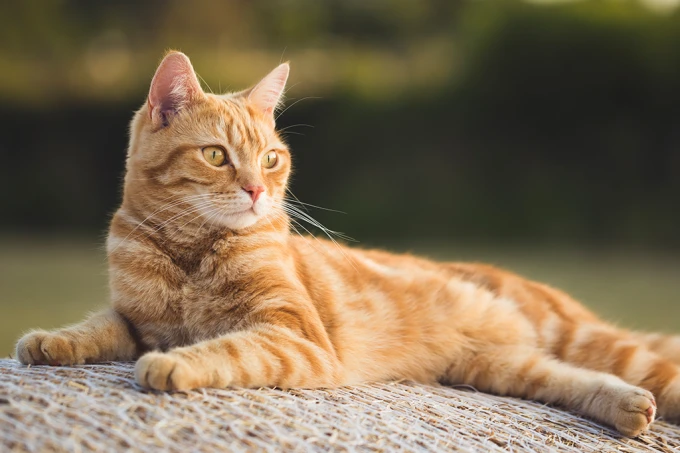
\includegraphics[width=3cm]{figuras/Gatos.png}}
                  \qquad
                  \subfigure[cachorros][Cachorros]{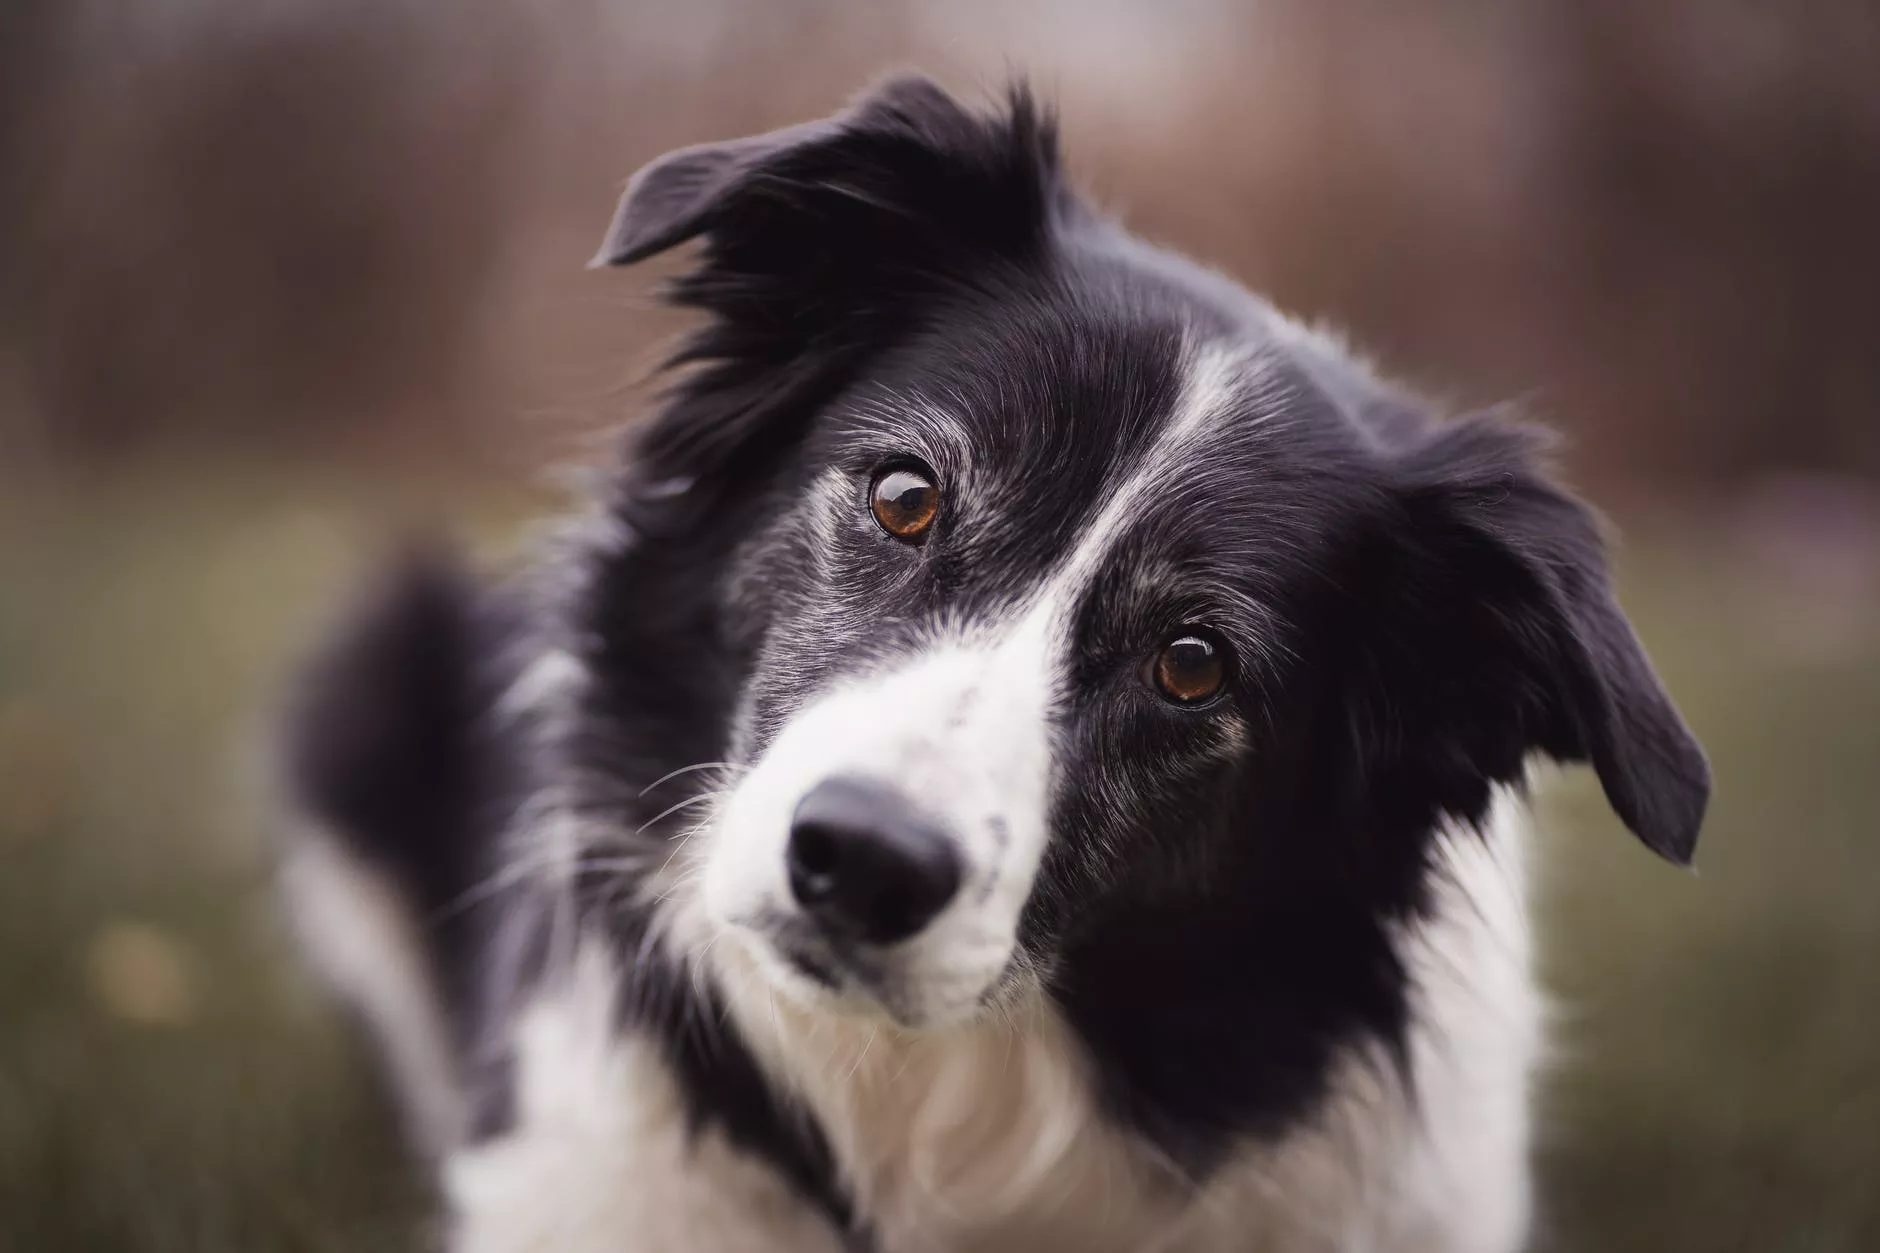
\includegraphics[width=3cm]{figuras/Cachorros.png}}
                  \qquad
                  \subfigure[morcegos][Morcegos]{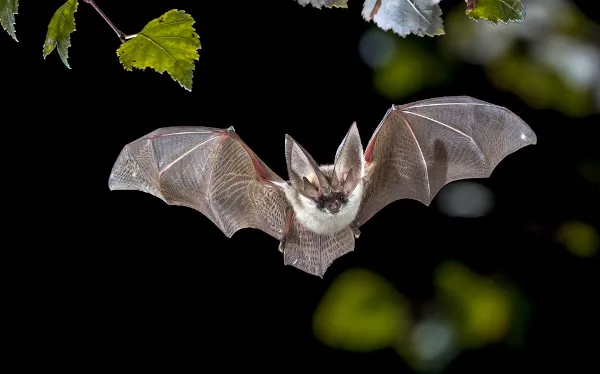
\includegraphics[width=2cm]{figuras/Morcegos.png}}
                  %\pause
              \end{figure}

              \vspace{0.3cm}
        \item E em relação aos humanos?
              %\pause

              \vspace{0.3cm}
        \item E por que o vírus é chamado de coronavírus?
              %\pause
              \vspace{0.3cm}

              \begin{figure}
                  \centering
                  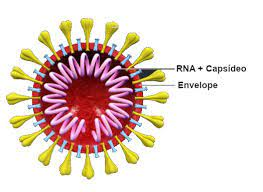
\includegraphics[width=3cm]{figuras/Coronavirus.jpg}
                  \caption{Coronavírus}
                  \label{fig:coronavirus}
              \end{figure}

    \end{enumerate}
\end{frame}

\begin{frame}{Pandemias causadas por coronavírus}

    No século XXI, o coronavírus já causou três pandemias \cite{tunas2020}.

    %\pause
    \vspace{0.5cm}

    \begin{table}[h]
        \begin{tabular}{|l|l|l|l|}
            \hline
            Vírus      & Casos                         & Óbitos    & Taxa de mortalidade      \\
            \hline
            SARS-CoV   & 8.000                         & 774       & 0.09675                  \\
            \hline
            MERS-CoV   & 2.494                         & 858       & \textcolor{red}{0.34681} \\
            \hline
            SARS-CoV-2 & \textcolor{blue}{696.943.378} & 6.931.505 & 0.0099                   \\
            \hline
        \end{tabular}
        \caption{\label{tab:corona}Comparações entre as pandemias \cite{tunas2020,cabral2020}}
    \end{table}
\end{frame}

\begin{frame}{Considerações sobre a COVID-19}

    \begin{enumerate}

        \item Nome do vírus;

              \vspace{0.4cm}


        \item Primeiro caso notificado;

              \vspace{0.4cm}

        \item Data de declaração como uma emergência de saúde de preocupação internacional;

              \vspace{0.4cm}

        \item Data de classificação como uma pandemia;

              \vspace{0.4cm}

        \item Início da vacinação contra a COVID-19 em vários países do mundo;

              \vspace{0.4cm}

        \item Começo do programa de vacinação contra a doença do novo coronavírus no Brasil.

    \end{enumerate}
\end{frame}

\section{Visão Geral sobre Modelos Epidêmicos}

\begin{frame}{Características dos Modelos Epidemiológicos}
    \begin{enumerate}

        \item Serão apresentados os modelos SI, SIS, SIR, SIRS e SEIR;

              \vspace{0.4cm}
              %\pause

        \item Estes modelos são compartimentados;

              \vspace{0.4cm}
              %\pause

        \item Nesses modelos, a população é

              \vspace{0.4cm}
              %\pause

              \begin{itemize}

                  \item Homogênea;

                        \vspace{0.4cm}

                  \item Fechada;

                        \vspace{0.4cm}

                  \item Sem dinâmica vital.

              \end{itemize}
    \end{enumerate}
\end{frame}

\begin{frame}{Variáveis e Parâmetros dos Modelos}
    \begin{enumerate}

        \item Variáveis:

              %\pause

              \begin{itemize}

                  \vspace{0.1cm}

                  \item $S \geq 0$ é a fração da população total chamada de suscetíveis;

                        \vspace{0.1cm}

                  \item $E \geq 0$ é a fração da população total chamada de expostos;

                        \vspace{0.1cm}

                  \item $I \geq 0$ é a fração da população total chamada de infectados;

                        \vspace{0.1cm}

                  \item $R \geq 0$ é a fração da população total chamada de recuperados.

              \end{itemize}

              \vspace{0.4cm}
              %\pause

        \item Parâmetros:
              %\pause

              \begin{itemize}

                  \item $\beta > 0$ é a taxa de infecção;

                        \vspace{0.1cm}


                  \item $\sigma > 0$ é a taxa de incubação;

                        \vspace{0.1cm}


                  \item $\lambda > 0$ é a taxa de perda de imunidade;

                        \vspace{0.1cm}


                  \item $\gamma > 0 $ é a taxa de recuperação.

              \end{itemize}

              \vspace{0.5cm}
              %\pause 

        \item A soma de todas as frações resulta na população total.

    \end{enumerate}
\end{frame}

\begin{frame}{Modelo SI}
    \begin{columns}
        \column{0.5\textwidth}
        \begin{figure}[ht]
            \centering
            \begin{tikzpicture}[auto, >=latex']
                \node [block, ] (s) {Suscetível \\ $S$};
                \node [block, right = 1 cm of s] (i) {Infectado \\ $I$};
                \draw [arrow] (s) -- node [above] {$\beta $} (i);
            \end{tikzpicture}
            \caption{\label{fig:modelSI}Fluxograma do Modelo SI.}
        \end{figure}
        $$\frac{dS}{dt} = -\beta SI,$$
        $$\frac{dI}{dt} = \beta SI,$$
        $$S + I = 1. $$
        \column{0.5\textwidth}
        \begin{figure}[ht]
            \center
            \subfigure[$I(0) = 0,1$ e $\beta = 0,1$.]{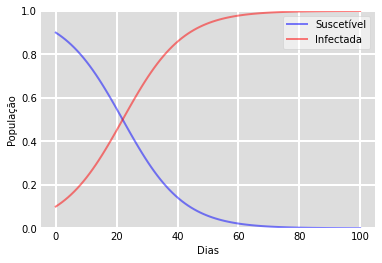
\includegraphics[width=4cm]{figuras/1ExemploSI.png}}
            \qquad
            \subfigure[$I(0) = 0,1$ e $\beta = 0,3$.]{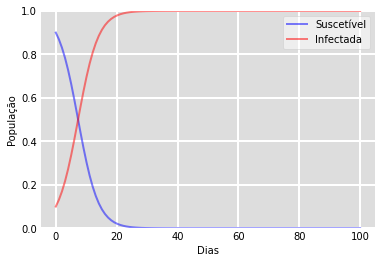
\includegraphics[width=4cm]{figuras/2ExemploSI.png}}
            \caption{\label{fig:exemplos_SI}Exemplos Numéricos do Modelo SI para Casos Novos.}
        \end{figure}
    \end{columns}
\end{frame}

\begin{frame}{Modelo SIS}
    \begin{columns}
        \column{0.5\textwidth}
        \begin{figure}
            \centering
            \begin{tikzpicture}[auto, >=latex']
                \node [block] (s) {Suscetível \\ $S$};
                \node [block, right = 1 cm of s] (i) {Infectado \\ $I$};
                \draw [->] (s) -- node [above] {$\beta$} (i);
                \draw [->, dashed] (i.north) |- ++(0cm,1.0cm) -- node [above, pos = 0.22mm] {$\gamma$} ++(-3cm,0cm) -| (s);
            \end{tikzpicture}
            \caption{\label{fig:modelSIS}Fluxograma do Modelo SIS.}
        \end{figure}
        $$\frac{dS}{dt} = -\beta SI + \gamma I,$$
        $$\frac{dI}{dt} = \beta SI - \gamma I,$$
        $$S + I = 1.$$
        \column{0.5\textwidth}
        \begin{figure}
            \centering
            \subfigure[$I(0) = 0.5$, $\beta = 0.1$ e $\gamma = 0.3$.]{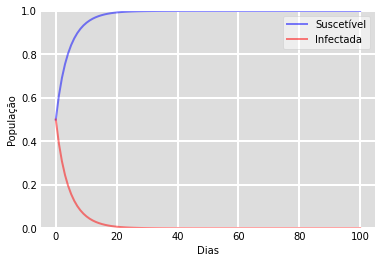
\includegraphics[width=4cm]{figuras/1ExemploSIS.png}}
            \subfigure[$I(0) = 0.5$, $\beta = 0.3$ e $\gamma = 0.1$.]{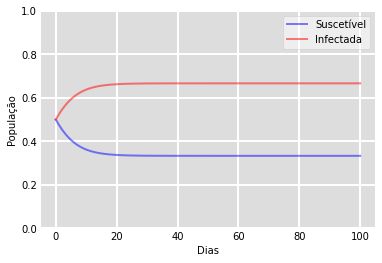
\includegraphics[width=4cm]{figuras/2ExemploSIS.png}}
            \caption{\label{fig:exemplos_SIS}Exemplos Numéricos do Modelo SIS para Casos Novos.}
        \end{figure}
    \end{columns}
\end{frame}

\begin{frame}{Modelo SIR}
    \begin{columns}
        \column{0.5\textwidth}
        \begin{figure}[ht]
            \scalebox{0.7}{
                \centering
                \begin{tikzpicture}[auto, >=latex']
                    \node [block, ] (s) {Suscetível \\ $S$};
                    \node [block, right = 1 cm of s] (i) {Infectado \\ $I$};
                    \node [block, right = 1 cm of i] (r) {Recuperado \\ $R$};
                    \draw [arrow] (s) -- node [above] {$\beta$} (i);
                    \draw [arrow] (i) -- node [above] {$\gamma$} (r);
                \end{tikzpicture}}
            \caption{\label{fig:modelSIR}Fluxograma do Modelo SIR para Casos Novos.}
        \end{figure}
        $$\frac{dS}{dt} = -\beta SI,$$
        $$\frac{dI}{dt} = \beta SI - \gamma I,$$
        $$\frac{dR}{dt} = \gamma I,$$
        $$S + I + R = 1.$$
        \column{0.5\textwidth}
        \begin{figure}[ht]
            \center
            \subfigure[$I(0) = 0,3$, $R(0) = 0$, $\beta = 0,2$ e $\gamma = 0,8 $.]{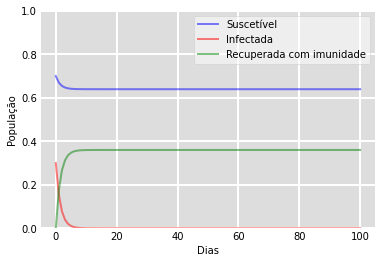
\includegraphics[width=3.5cm]{figuras/1ExemploSIR.png}}
            \qquad
            \subfigure[$I(0) = 0,3$, $R(0) = 0$, $\beta = 0,8$ e $\gamma = 0,2$.]{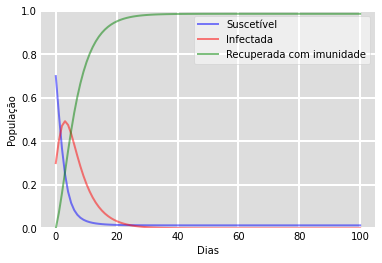
\includegraphics[width=3.5cm]{figuras/2ExemploSIR.png}}
            \caption{\label{fig:exemplos_SIR}Exemplos Numéricos do Modelo SIR para Casos Novos.}
        \end{figure}
    \end{columns}
\end{frame}

\begin{frame}{Modelo SIRS}
    \begin{columns}
        \column{0.5\textwidth}
        \begin{figure}[ht]
            \scalebox{0.7}{
                \centering
                \begin{tikzpicture}[auto, >=latex']
                    \node [block, ] (s) {Suscetível \\ $S$};
                    \node [block, right = 1 cm of s] (i) {Infectado \\ $I$};
                    \node [block, right = 1 cm of i] (r) {Recuperado \\ $R$};
                    \draw [arrow] (s) -- node [above] {$\beta$} (i);
                    \draw [arrow] (i) -- node [above] {$\gamma$} (r);
                    \draw [arrow] (r.north) |- ++(0cm,+1.0cm) -- node [above, pos = 0.45mm] {$\lambda$} ++(-3cm,0cm) -| (s);
                \end{tikzpicture}}
            \caption{\label{fig:modelSIRS}Fluxograma do Modelo SIRS.}
        \end{figure}
        $$\frac{dS}{dt} = -\beta SI + \lambda R,$$
        $$\frac{dI}{dt} = \beta SI - \gamma I, $$
        $$\frac{dR}{dt} = \gamma I - \lambda R,$$
        $$ S + I + R = 1.$$
        \column{0.5\textwidth}
        \begin{figure}[ht]
            \center
            \subfigure[$I(0) = 0,2$, $R(0) = 0$, $\beta = 0,2$, $\lambda = 0,4$ e $\gamma = 0,8$.]{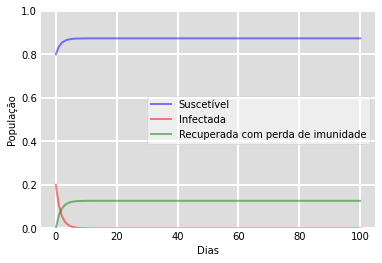
\includegraphics[width=3.5cm]{figuras/1ExemploSIRS.png}}
            \qquad
            \subfigure[$I(0) = 0,2$, $R(0) = 0$, $\beta = 0,8$, $\lambda = 0,2$ e      $\gamma =  0.5$.]{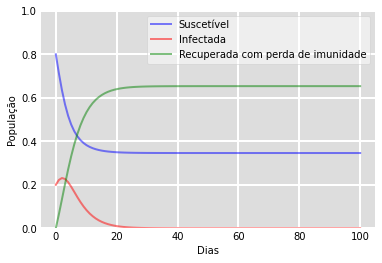
\includegraphics[width=3.5cm]{figuras/2ExemploSIRS.png}}
            \caption{\label{fig:exemplos_SIRS}Exemplos Numéricos do Modelo SIRS para Casos Novos.}
        \end{figure}
    \end{columns}
\end{frame}

\begin{frame}{Modelo SEIR}
    \begin{columns}
        \column{0.5\textwidth}
        \begin{figure}[ht]
            \scalebox{0.6}{
                \centering
                \begin{tikzpicture}[auto, >=latex']
                    \node [block, ] (s) {Suscetível \\ $S$};
                    \node [block, right = 1 cm of s] (e) {Exposto \\ $E$};
                    \node [block, right = 1 cm of e] (p) {Infectado \\ $I$};
                    \node [block, right = 1 cm of p] (r) {Recuperado \\ $R$};
                    \draw [arrow] (s) -- node [above] {$\beta$} (e);
                    \draw [arrow] (e) -- node [above] {$\sigma$} (p);
                    \draw [arrow] (p) -- node [above] {$\gamma$} (r);
                \end{tikzpicture}}
            \caption{\label{fig:modelSEIR}Fluxograma do Modelo SEIR.}
        \end{figure}
        $$\frac{dS}{dt} = -\beta SI,$$
        $$\frac{dE}{dt} = \beta SI - \sigma E,$$
        $$\frac{dI}{dt} = - \gamma I + \sigma E,$$
        $$\frac{dR}{dt} = \gamma I,$$
        $$ S + E + I + R = 1.$$
        \column{0.5\textwidth}
        \begin{figure}[ht]
            \center
            \subfigure[$E(0) = 0,3$, $I(0) = 0,1$, $R(0) = 0$, $\beta = 0,1$, $\sigma = 0,4$ e $\gamma = 0,3$.]{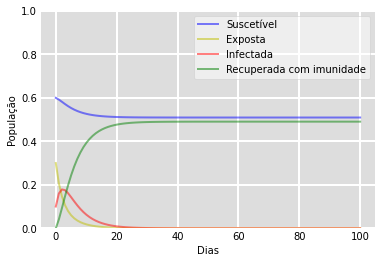
\includegraphics[width=3.0cm]{figuras/1ExemploSEIR.png}}
            \qquad
            \subfigure[$E(0) = 0,3$, $I(0) = 0,1$, $R(0) = 0$, $\beta = 0,3$, $\sigma = 0,4$ e $\gamma = 0,1 $.]{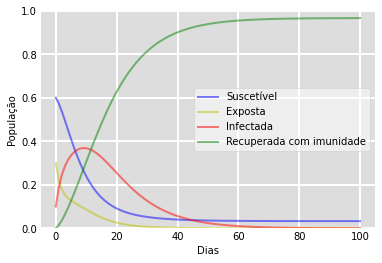
\includegraphics[width=3.0cm]{figuras/2ExemploSEIR.png}}
            \caption{\label{fig:exemplos_SEIR}Exemplos Numéricos do Modelo SEIR para Casos Novos.}
        \end{figure}
    \end{columns}
\end{frame}

\section{Revisão Sistemática}
\begin{frame}{Identificação dos Trabalhos Publicados}
    \begin{itemize}
        \item Doenças Infecciosas Virais
              \begin{itemize}
                  \item Pacote \textit{Bibliometrix} na Linguagem R;
                  \item Descritor de busca: ((mathematical $\lor$ sir) $\land$ model) $\land$ (sars-cov-2 $\lor$ covid-19);
                  \item Intervalo de Tempo: 2019 a 2024;
                  \item
              \end{itemize}
    \end{itemize}
\end{frame}

\begin{frame}{Fluxograma}
    \begin{figure}[htbp]
        \scalebox{0.7}{
        \centering
        % Define block styles
        \tikzstyle{block} = [rectangle, draw, fill=white,
        text width=20em, text centered, rounded corners, node distance=2cm, minimum height=2em]
        \tikzstyle{line} = [draw, -latex]
        \tikzstyle{cloud} = [draw, ellipse,fill=white, node distance=2cm,
        minimum height=2em]
        \begin{tikzpicture}[node distance = 3cm, auto]
            % Place nodes
            \node [block] (observacao) {Total de manuscritos encontrados: 13.041};
            \node [block, below of = observacao] (acesso) {\textit{Scopus}: 7.802 \\ \textit{Web of Science}: 4.653 \\ \textit{PubMed}: 2.686};
            \node [block, below of = acesso] (foco) {Após a remoção das duplicatas, ficaram xxxx documentos};
            \node [block, below of = foco]   (dado) {Após a exclusão dos trabalhos não escritos na língua inglesa, restaram xxxx documentos};
            % Draw edges
            \path [line] (observacao) -- (acesso);
            \path [line] (acesso)   -- (foco);
            \path [line] (foco)   -- (dado);
        \end{tikzpicture}}
        \caption{\label{fig:fluxograma}Fluxograma do processo de triagem para inclusão dos trabalhos na revisão sistemática.}
    \end{figure}
\end{frame}

\begin{frame}{Produção Científica}
    \begin{figure}[ht]
        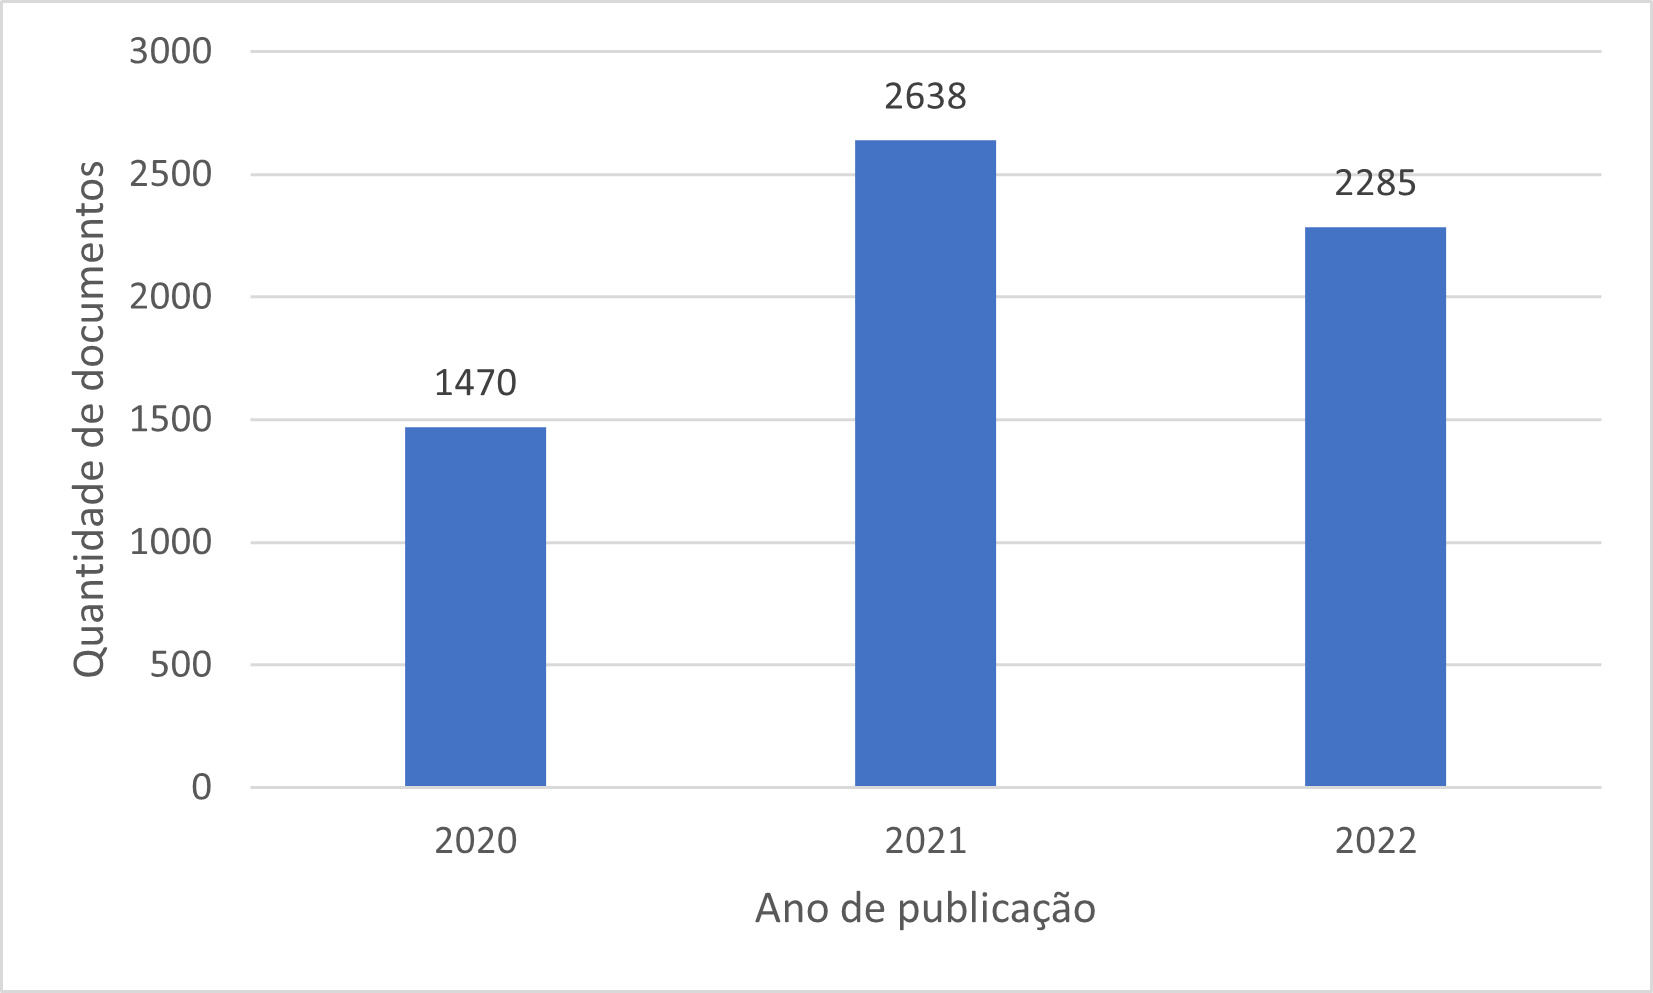
\includegraphics[width=7cm]{figuras/artigosano.png}
        \caption{\label{fig:ano}Quantidade de documentos publicados por ano}
    \end{figure}
\end{frame}

\begin{frame}{Local de Publicações}
    \begin{table}[htbp]
        \scalebox{0.6}{
            \centering
            \begin{tabular}{|c|c|}
                \hline
                País                      & Quantidade de documentos \\
                \hline
                Estados Unidos da América & 725                      \\
                \hline
                China                     & 609                      \\
                \hline
                Índia                     & 437                      \\
                \hline
                Reino Unido               & 286                      \\
                \hline
                Itália                    & 219                      \\
                \hline
                Arábia Saudita            & 173                      \\
                \hline
                Brasil                    & 168                      \\
                \hline
                Canadá                    & 161                      \\
                \hline
                Espanha                   & 133                      \\
                \hline
                França                    & 131                      \\
                \hline
            \end{tabular}}
        \caption{\label{tab:localpubli}As dez nações com maior produção científica}
    \end{table}

    \begin{table}[htbp]
        \centering
        \scalebox{0.8}{
            \begin{tabular}{|c|c|}
                \hline
                Continente & Quantidade de documentos \\
                \hline
                Asiático   & 1219                     \\
                \hline
                Americano  & 1054                     \\
                \hline
                Europeu    & 769                      \\
                \hline
            \end{tabular}}
        \caption{\label{tab:continente}Os continentes dos dez países com maior produção científica}
    \end{table}
\end{frame}

\begin{frame}{Palavras-Chave}
    \begin{table}[htbp]
        \centering
        \begin{tabular}{|c|c|}
            \hline
            Palavra-chave                      & Número de ocorrências \\
            \hline
            \textit{covid-19}                  & 2912                  \\
            \hline
            \textit{sars-cov-2}                & 604                   \\
            \hline
            \textit{mathematical model}        & 416                   \\
            \hline
            \textit{sir model}                 & 308                   \\
            \hline
            \textit{coronavirus}               & 299                   \\
            \hline
            \textit{epidemiology}              & 249                   \\
            \hline
            \textit{mathematical modeling}     & 242                   \\
            \hline
            \textit{basic reproduction number} & 228                   \\
            \hline
            \textit{pandemic}                  & 217                   \\
            \hline
            \textit{mathematical modelling}    & 195                   \\
            \hline
        \end{tabular}
        \caption{\label{tab:palcha}As dez palavras-chave mais relevantes}
    \end{table}
\end{frame}

\section{Métodos Computacionais}
\begin{frame}{Identificação dos Métodos Computacionais}
    \begin{itemize}
        \item Pacote \textit{Bibliometrix} na Linguagem R;
              \vspace{0.1cm}
        \item Descritor de busca: ((sir $\land$ model) $\land$ (sars-cov-2 $\lor$ covid-19) $\land$ ((estimation $\lor$ estimating) $\land$ parameters))).
    \end{itemize}
    \begin{figure}[htbp]
        \scalebox{0.7}{
        \centering
        % Define block styles
        \tikzstyle{block} = [rectangle, draw, fill=white,
        text width=20em, text centered, rounded corners, node distance=2cm, minimum height=2em]
        \tikzstyle{line} = [draw, -latex]
        \tikzstyle{cloud} = [draw, ellipse,fill=white, node distance=2cm,
        minimum height=2em]

        \begin{tikzpicture}[node distance = 3cm, auto]
            % Place nodes
            \node [block] (observacao) {Total de publicações encontradas: 370};
            \node [block, below of = observacao] (acesso) {\textit{Web of Science}: 173  \\ \textit{Scopus}: 146 \\ \textit{PubMed}: 51};
            \node [block, below of = acesso] (foco) {Após a remoção das duplicatas, restaram 157 trabalhos publicados};
            \node [block, below of = foco]   (dado) {Após a exclusão dos trabalhos não escritos na língua inglesa, ficaram 156 artigos};
            % Draw edges
            \path [line] (observacao) -- (acesso);
            \path [line] (acesso)   -- (foco);
            \path [line] (foco)   -- (dado);
        \end{tikzpicture}}
        \caption{\label{fig:fluxogramaBusca}Fluxograma do processo de triagem para identificação dos trabalhos publicados pela nova busca.}
    \end{figure}
\end{frame}

\begin{frame}{Principais Artigos}
    \begin{table}[htbp]
        \scalebox{0.55}{
            \centering
            \begin{tabular}{|p{4cm}|c|c|p{4cm}|}
                \hline
                Título                                                                                                                      & Autores              & Ano de Publicação & Métodos                                                     \\
                \hline
                \textit{Estimating SIR model parameters from data using differential evolution: an application with COVID-19 data}          & \cite{rica2020}      & 2020              & Evolução Diferencial e Busca Aleatória                      \\
                \hline
                \textit{A modified variable-order fractional SIR model to predict the spread of COVID-19 in India}                          & \cite{singh2021}     & 2021              & Evolução Diferencial                                        \\
                \hline
                \textit{Parameter Estimation of Compartmental Epidemiological Model Using Harmony Search Algorithm and Its Variants}        & \cite{gopal2021}     & 2021              & Busca Harmônica                                             \\
                \hline
                \textit{Estimating Effective Reproduction Number for SIR Compartmental Model: A Stochastic Evolutionary Approach}           & \cite{wong2022}      & 2022              & Evolução Diferencial e \textit{Particle Swarm Optimization} \\
                \hline
                \textit{A Comparative Study on Parameter Estimation of COVID Epidemiological Models Using Differential Evolution Algorithm} & \cite{panigrahi2022} & 2022              & Evolução Diferencial                                        \\
                \hline

                \hline
            \end{tabular}}
        \caption{\label{tab:busca_metodos}Métodos de Inteligência Computacional identificados nos principais trabalhos.}
    \end{table}
\end{frame}
\section{Experimentos Computacionais}

\begin{frame}{Base de dados da COVID-19}
    \begin{itemize}
        \item A obtenção dos dados de casos acumulados e novos de COVID-19 em duas regiões, Ceará (CE) e Brasil (BR), foi realizada por meio da coleta de informações do Ministério da Saúde.

              \vspace{0.2cm}

        \item Os dados coletados abrangem um período de três anos, o que equivale a 1.095 dias para o Estado do Ceará, iniciando em 17 de março de 2020 e concluindo em 16 de março de 2023.

              \vspace{0.2cm}

        \item Os dados coletados para o Brasil compreendem 1.096 dias, correspondendo a um período de três anos, com início em 26 de fevereiro de 2020 e encerramento em 25 de fevereiro de 2023.

              \vspace{0.2cm}

        \item Duas alterações nos dados ocorreram devido a mudanças nos valores:

              \vspace{0.2cm}

              \begin{itemize}
                  \item Negativos

                        \vspace{0.2cm}

                  \item Nulos
              \end{itemize}
    \end{itemize}
\end{frame}

\begin{frame}{Modelo SIR com 3 Equações Diferenciais}
    $$\frac{d}{dt}S(t) = -\beta \cdot S(t) \cdot I(t),$$
    $$\frac{dI}{dt}I(t) = \beta \cdot S(t) \cdot I(t) - \alpha \cdot I(t),$$
    $$\frac{d}{dt}R(t) = \alpha \cdot I(t),$$
    $$S(t_0) = S_0, \text{ } I(t_0) = I_0, \text{ } R(t_0) = R_0,$$
    $$S(t) + I(t) + R(t) = N.$$
    \begin{itemize}
        \item  $S(t)$ o número de indivíduos suscetíveis no tempo $t$; $I(t)$ o número cumulativo de indivíduos infectados no instante $t$; $R(t)$ o número de indivíduos recuperados no instante $t$; $\alpha$ a taxa de recuperação; $\beta$ a taxa de transmissão; $t_0$ o tempo inicial; $S(t_0)$ o número de indivíduos suscetíveis em $t_0$; $I(t_0)$ o número de casos acumulados de infectados em $t_0$; $R(t_0)$ o número de casos recuperados em $t_0$.
    \end{itemize}
\end{frame}

\begin{frame}{Modelo SIR com 2 Equações Diferenciais}
    Calculando $R(t) = N - S(t) - I(t)$, tem-se que
    \begin{equation}
        \label{eq:ed1}
        \begin{aligned}
            \frac{d}{dt}S(t) & = -\beta \cdot S(t) \cdot I(t),                     \\
            \frac{d}{dt}I(t) & = -\alpha \cdot I(t) + \beta \cdot S(t) \cdot I(t), \\
            S(t_0)           & = S_0,                                              \\
            I(t_0)           & = I_0.
        \end{aligned}
    \end{equation}
    \begin{itemize}
        \item $S(t)$ o número de indivíduos suscetíveis no instante $t$; $I(t)$ o número acumulado de indivíduos infectados no instante t; $\alpha$ a taxa de recuperação; $\beta$ a taxa de transmissão; $t_0$ o tempo inicial; $S(t_0)$ o número de indivíduos suscetíveis no tempo inicial $t_0$; $I(t_0)$ o número de casos acumulados de infectados no tempo inicial $t_0$.
    \end{itemize}
\end{frame}

\begin{frame}{Modelo SIR com 1 Equação Diferencial}
    Por \cite{rica2020}, tem-se que
    \begin{equation}
        \label{eq:ed2}
        \begin{aligned}
            \frac{d}{dt}v(t) & = -\alpha \cdot v(t) + \nu \cdot \xi_0 \cdot (1 - \exp({
            \frac{\alpha}{\nu}v(t)})) + I_0,                                            \\
            v(t_0)           & = 0.
        \end{aligned}
    \end{equation}
    \begin{itemize}
        \item $v(t)$ o número cumulativo de casos infectados no tempo $t$; $v(t_0)$ o número de casos acumulados de infectados no instante inicial $t_0$; $\alpha$ a taxa de recuperação; $\beta$ a taxa de transmissão; $\nu = \frac{\alpha}{\beta}$; $t_0$ o instante inicial; $I_0$ o número de casos infectados no instante inicial $t_0$; $\xi_0$ o número de reprodução no instante inicial $t_0$.
    \end{itemize}
\end{frame}

\begin{frame}{Estimação dos Parâmetros}
    \begin{table}[htbp]
        \centering
        \begin{tabular}{|c|c|}
            \hline
            Parâmetro & Intervalo \\
            \hline
            $\alpha$  & [0.0,1.0] \\
            \hline
            $\beta$   & [0.0,1.0] \\
            \hline
        \end{tabular}
        \caption{\label{tab:param_model2}Limites Inferiores e Superiores do Modelo \ref{eq:ed1}.}
    \end{table}

    \begin{table}[htbp]
        \centering
        \begin{tabular}{|c|c|}
            \hline
            Parâmetro & Intervalo    \\
            \hline
            $\alpha$  & [0.001,0.1]  \\
            \hline
            $\nu$     & [1000,30000] \\
            \hline
            $t_0$     & [1,50]       \\
            \hline
            $I_0$     & [0,30]       \\
            \hline
            $\xi_0$   & [1,7]        \\
            \hline
        \end{tabular}
        \caption{\label{tab:param_model1}Limites Inferiores e Superiores do Modelo \ref{eq:ed2}.}
    \end{table}
\end{frame}

\begin{frame}{Estimação dos Parâmetros}
    \begin{itemize}
        \item Uma semente comum foi utilizada para a geração de números pseudoaleatórios nos métodos BAG, BAL, BH, ED e PSO.
        \item Ao utilizar esses métodos, torna-se viável a estimativa dos parâmetros dos Modelos \ref{eq:ed1} e \ref{eq:ed2}. Esse processo é efetuado por meio de uma função objetivo que visa a minimização do erro quadrático médio entre $v_{n}$ e $v(t_n)$. Essa função pode ser expressa da seguinte forma:
              $$ min \text{ } f(v) = \sum_{n=0}^{N-1} (v_n - v(t_n))^2.$$
    \end{itemize}
\end{frame}

\begin{frame}{Estimação dos Parâmetros}
    \begin{table}[htbp]

        \centering
        \scalebox{0.6}{
            \begin{tabular}{|c|p{4cm}|}
                \hline
                Método                              & Inicialização dos Parâmetros de Controle                               \\
                \hline
                Busca Aleatória Global              & $N_p = 1$ e $N_{max} = 1000$                                           \\
                \hline
                Busca Aleatória Local               & $N_p = 1$ e $N_{max} = 1000$                                           \\
                \hline
                Busca Harmônica                     & $HMS = 15$, $HMCR = 0.99$, $PAR = 0.01$, $BW = 0.01$ e $MaxImp = 1000$ \\
                \hline
                Evolução Diferencial                & $N_p = 15$, $F = U[0.5,1]$, $C_r = 0.7$ e $G_{max} = 1000$             \\
                \hline
                Otimização por Enxame de Partículas & $N_p = 15$, $w = 0.5$, $c_1 = 2$, $c_2 = 2$ e $N_{max} = 1000$         \\
                \hline
            \end{tabular}}
        \caption{\label{tab:inicializar_metodos}Inicialização dos parâmetros de controle dos métodos.}
    \end{table}
    \begin{itemize}
        \item $N_p$ o tamanho da população; $N_{max}$ o número máximo de iterações;
              $HMS$ o tamanho da memória harmônica; $HMCR$ a taxa de consideração da memória harmônica; $PAR$ o ajuste de altura do tom; $BW$ a largura de banda; $MaxIm$ o número máximo de improvisações; $F$ é o fator de mutação para cada geração; $C_r$ é a constante de cruzamento para cada geração; $G_{max}$ o número máximo de gerações; $w$ o fator de inércia; $c_1$ o coeficiente cognitivo da velocidade; $c_2$ o coeficiente social da velocidade.
    \end{itemize}
\end{frame}
\begin{frame}{Período de Análise para o Ceará}
    \begin{table}[htbp]
        \centering
        \begin{tabular}{|c|c|c|c|}
            \hline
            Data Inicial & Data Final & Número de dias \\
            \hline
            17/03/2020   & 16/03/2023 & 1095           \\
            \hline
        \end{tabular}
        \caption{\label{tab:ceto}Período de análise para o Ceará.}
    \end{table}

    \begin{table}[htbp]
        \centering
        \begin{tabular}{|c|c|c|c|}
            \hline
            Ano & Data Inicial & Data Final & Número de dias \\
            \hline
            1   & 17/03/2020   & 16/03/2021 & 365            \\
            \hline
            2   & 17/03/2021   & 16/03/2022 & 365            \\
            \hline
            3   & 17/03/2022   & 16/03/2023 & 365            \\
            \hline
        \end{tabular}
        \caption{\label{tab:cea}Partição anual do período completo para o Ceará.}
    \end{table}
\end{frame}

\begin{frame}{Período de Análise para o Ceará}
    \begin{table}[htbp]
        \centering
        \begin{tabular}{|c|c|c|c|}
            \hline
            Semestre & Data Inicial & Data Final & Número de dias \\
            \hline
            1        & 17/03/2020   & 16/09/2020 & 184            \\
            \hline
            2        & 17/09/2020   & 16/03/2021 & 181            \\
            \hline
            3        & 17/03/2021   & 16/09/2021 & 184            \\
            \hline
            4        & 17/09/2021   & 16/03/2022 & 181            \\
            \hline
            5        & 17/03/2022   & 16/09/2022 & 184            \\
            \hline
            6        & 17/09/2022   & 16/03/2023 & 181            \\
            \hline
        \end{tabular}
        \caption{\label{tab:ces}Partição semestral do período completo para o Ceará.}
    \end{table}
\end{frame}

\begin{frame}{Período de Análise para o Ceará}
    \begin{table}[htbp]
        \centering
        \begin{tabular}{|c|c|c|c|}
            \hline
            Trimestre & Data Inicial & Data Final & Número de dias \\
            \hline
            1         & 17/03/2020   & 16/06/2020 & 92             \\
            \hline
            2         & 17/06/2020   & 16/09/2020 & 92             \\
            \hline
            3         & 17/09/2020   & 16/12/2020 & 91             \\
            \hline
            4         & 17/12/2020   & 16/03/2021 & 90             \\
            \hline
            5         & 17/03/2021   & 16/06/2021 & 92             \\
            \hline
            6         & 17/06/2021   & 16/09/2021 & 92             \\
            \hline
            7         & 17/09/2021   & 16/12/2021 & 91             \\
            \hline
            8         & 17/12/2021   & 16/03/2022 & 90             \\
            \hline
            9         & 17/03/2022   & 16/06/2022 & 92             \\
            \hline
            10        & 17/06/2022   & 16/09/2022 & 92             \\
            \hline
            11        & 17/09/2022   & 16/12/2022 & 91             \\
            \hline
            12        & 17/12/2022   & 16/03/2023 & 90             \\
            \hline
        \end{tabular}
        \caption{\label{tab:cetr}Partição trimestral do período completo para o Ceará.}
    \end{table}
\end{frame}

\begin{frame}{Resultados das Simulações Numéricas para o Ceará}
    \begin{figure}[ht]
        \center
        \subfigure[Busca Aleatória Global]{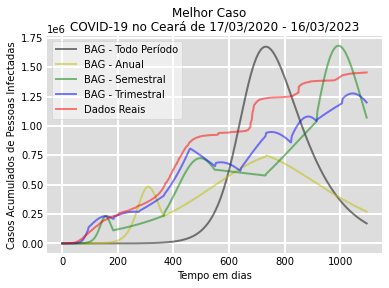
\includegraphics[width=3cm]{figuras/2BAGCE1.png}}
        \qquad
        \subfigure[Busca Aleatória Local]{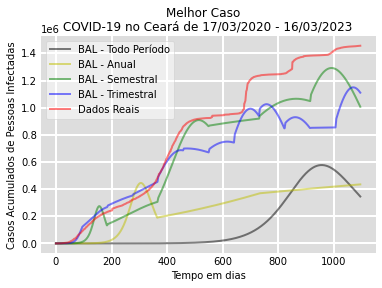
\includegraphics[width=3cm]{figuras/2BALCE1.png}}
        \qquad
        \subfigure[Busca Harmônica]{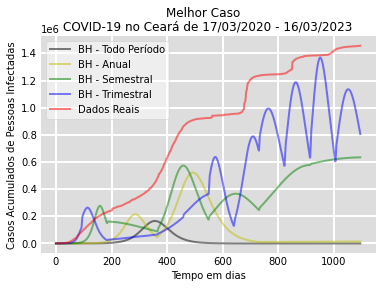
\includegraphics[width=3cm]{figuras/2BHCE1.png}}
        \qquad
        \subfigure[Evolução Diferencial]{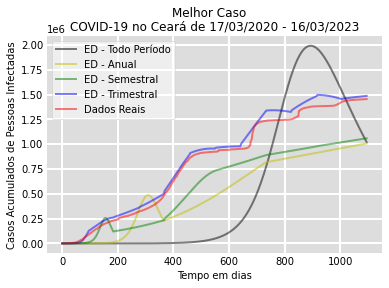
\includegraphics[width=3cm]{figuras/2EDCE1.png}}
        \qquad
        \subfigure[\textit{Particle Swarm Optimization}]{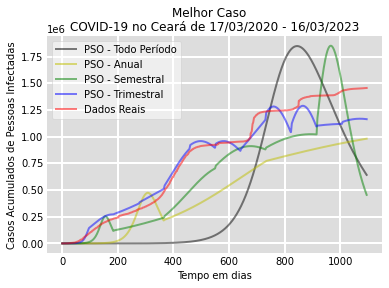
\includegraphics[width=3cm]{figuras/2PSOCE1.png}}
        \caption{\label{fig:MetodosIsoladosMelhorCasoModelo2Ceara}Gráficos de Melhor Caso para o Modelo \ref{eq:ed1}.}
    \end{figure}
\end{frame}

\begin{frame}{Resultados das Simulações Numéricas para o Ceará}
    \begin{figure}[ht]
        \center
        \subfigure[Busca Aleatória Global]{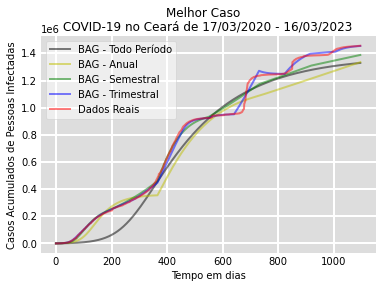
\includegraphics[width=3cm]{figuras/BAGCE1.png}}
        \qquad
        \subfigure[Busca Aleatória Local]{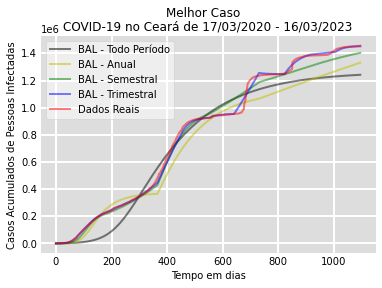
\includegraphics[width=3cm]{figuras/BALCE1.png}}
        \qquad
        \subfigure[Busca Harmônica]{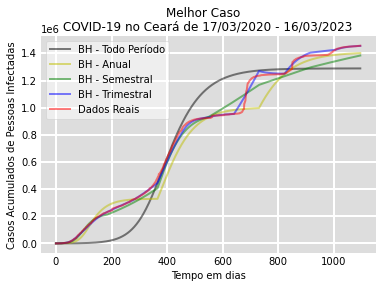
\includegraphics[width=3cm]{figuras/BHCE1.png}}
        \qquad
        \subfigure[Evolução Diferencial]{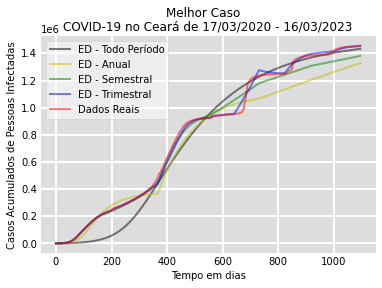
\includegraphics[width=3cm]{figuras/EDCE1.png}}
        \qquad
        \subfigure[\textit{Particle Swarm Optimization}]{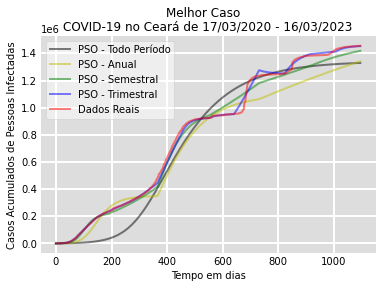
\includegraphics[width=3cm]{figuras/PSOCE1.png}}
        \caption{\label{fig:MetodosIsoladosMelhorCasoModelo1Ceara}Gráficos de Melhor Caso para o Modelo \ref{eq:ed2}.}
    \end{figure}
\end{frame}

\begin{frame}{Resultados das Simulações Numéricas para o Ceará}
    \begin{figure}[ht]
        \center
        \subfigure[Modelo 1]{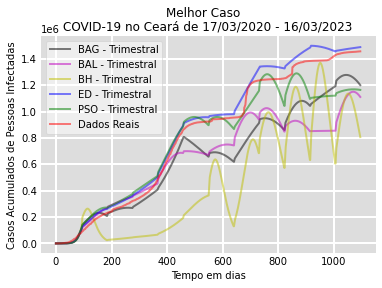
\includegraphics[width=5cm]{figuras/Exc25.png}}
        \qquad
        \subfigure[Modelo 2]{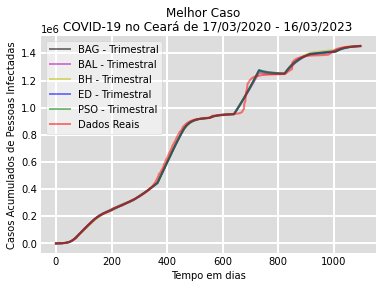
\includegraphics[width=5cm]{figuras/Exc27.png}}
        \caption{\label{fig:MetodosJuntosMelhorCasoCeara}Comparação entre os Modelos SIR no Melhor Caso.}
    \end{figure}
\end{frame}

\begin{frame}{Resultados das Simulações Numéricas para o Ceará}
    \begin{figure}[ht]
        \center
        \subfigure[Busca Aleatória Global]{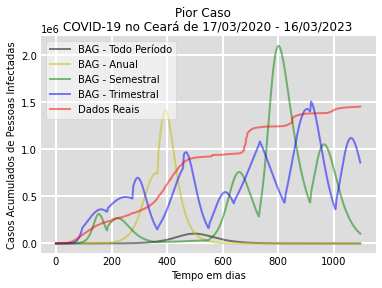
\includegraphics[width=3cm]{figuras/2BAGCE2.png}}
        \qquad
        \subfigure[Busca Aleatória Local]{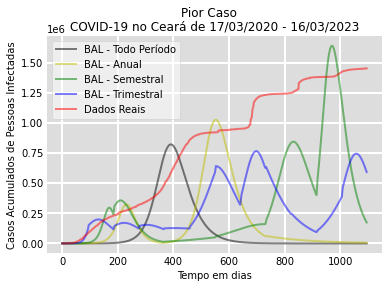
\includegraphics[width=3cm]{figuras/2BALCE2.png}}
        \qquad
        \subfigure[Busca Harmônica]{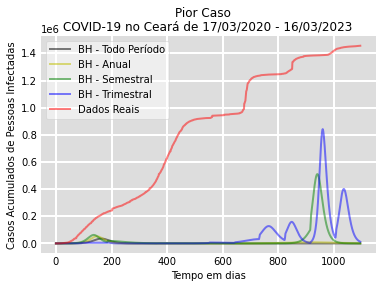
\includegraphics[width=3cm]{figuras/2BHCE2.png}}
        \qquad
        \subfigure[Evolução Diferencial]{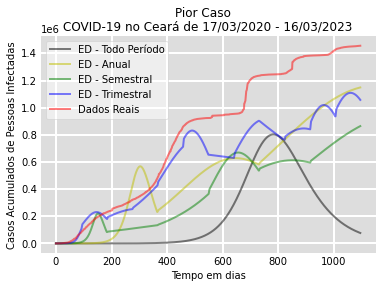
\includegraphics[width=3cm]{figuras/2EDCE2.png}}
        \qquad
        \subfigure[\textit{Particle Swarm Optimization}]{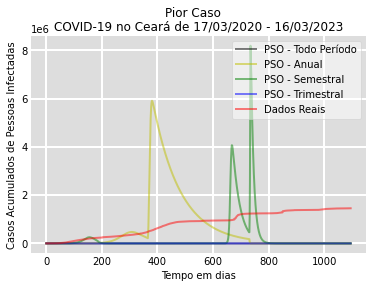
\includegraphics[width=3cm]{figuras/2PSOCE2.png}}
        \caption{\label{fig:MetodosIsoladosPiorCasoModelo2Ceara}Gráficos de Pior Caso para o Modelo \ref{eq:ed1}.}
    \end{figure}
\end{frame}

\begin{frame}{Resultados das Simulações Numéricas para o Ceará}
    \begin{figure}[ht]
        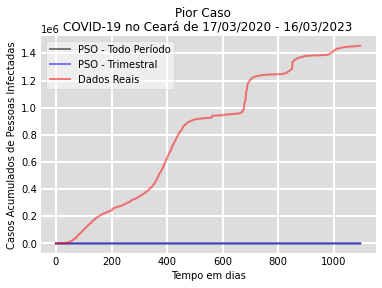
\includegraphics[width=5cm]{figuras/PSOCE5.png}
        \caption{\label{fig:psoce5}Novo Gráfico de Pior Caso do Método PSO para o Modelo \ref{eq:ed1}.}
    \end{figure}
\end{frame}

\begin{frame}{Resultados das Simulações Numéricas para o Ceará}
    \begin{figure}[ht]
        \center
        \subfigure[Busca Aleatória Global]{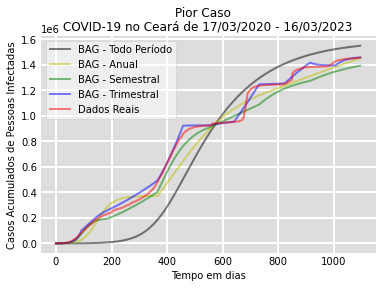
\includegraphics[width=3cm]{figuras/BAGCE2.png}}
        \qquad
        \subfigure[Busca Aleatória Local]{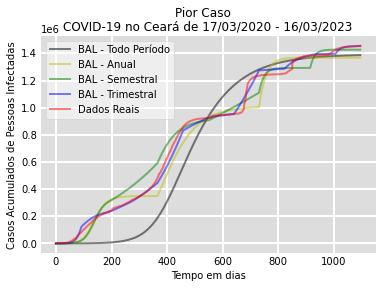
\includegraphics[width=3cm]{figuras/BALCE2.png}}
        \qquad
        \subfigure[Busca Harmônica]{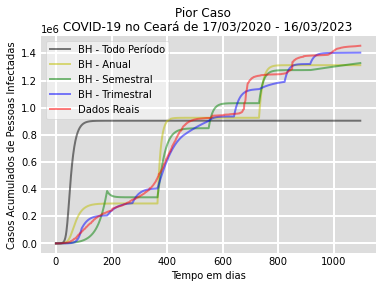
\includegraphics[width=3cm]{figuras/BHCE2.png}}
        \qquad
        \subfigure[Evolução Diferencial]{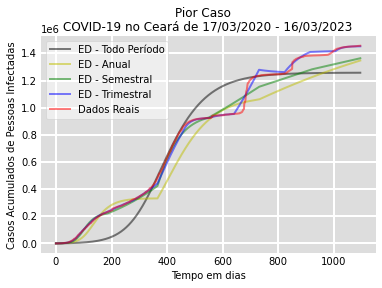
\includegraphics[width=3cm]{figuras/EDCE2.png}}
        \qquad
        \subfigure[\textit{Particle Swarm Optimization}]{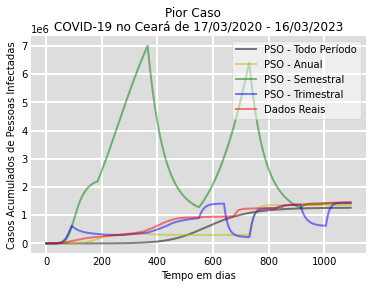
\includegraphics[width=3cm]{figuras/PSOCE2.png}}
        \caption{\label{fig:MetodosIsoladosPiorCasoModelo1Ceara}Gráficos de Pior Caso para o Modelo \ref{eq:ed2}.}
    \end{figure}
\end{frame}

\begin{frame}{Resultados das Simulações Numéricas para o Ceará}
    \begin{figure}[ht]
        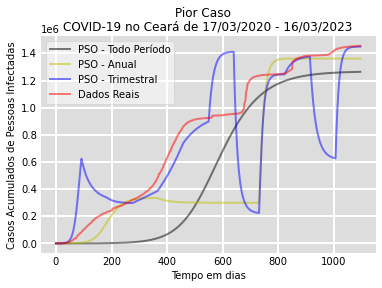
\includegraphics[width=6cm]{figuras/PSOCE4.png}
        \caption{\label{fig:psoce4}Novo Gráfico de Pior Caso do Método PSO para o Modelo \ref{eq:ed2}.}
    \end{figure}
\end{frame}

\begin{frame}{Resultados das Simulações Numéricas para o Ceará}
    \begin{figure}[ht]
        \center
        \subfigure[Modelo 1]{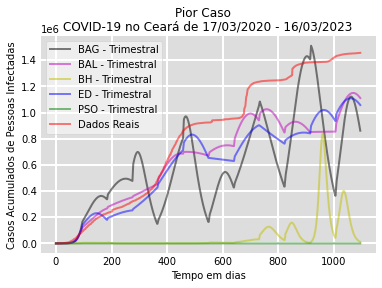
\includegraphics[width=5cm]{figuras/Exc26.png}}
        \qquad
        \subfigure[Modelo 2]{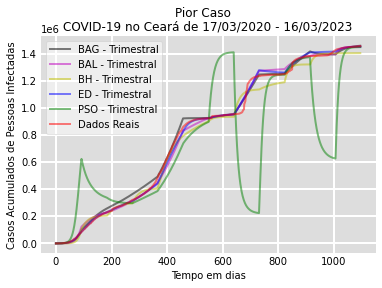
\includegraphics[width=5cm]{figuras/Exc20.png}}
        \caption{\label{fig:MetodosJuntosPiorCasoCeara}Comparação entre os Modelos SIR no Pior Caso.}
    \end{figure}
\end{frame}

\begin{frame}{Resultados das Simulações Numéricas para o Ceará}
    \begin{figure}[ht]
        \center
        \subfigure[Exclusão do Método PSO]{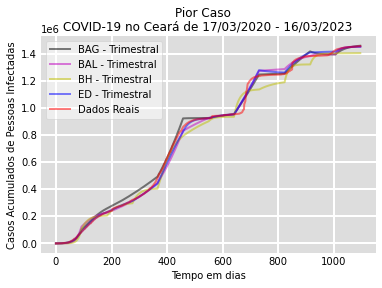
\includegraphics[width=3.5cm]{figuras/Exc21.png}}
        \qquad
        \subfigure[Exclusão do Método BH]{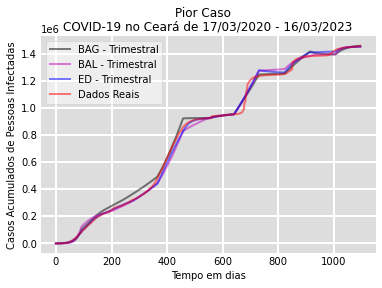
\includegraphics[width=3.5cm]{figuras/Exc22.png}}
        \qquad
        \subfigure[Exclusão do Método BAG]{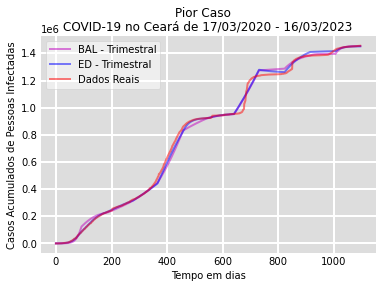
\includegraphics[width=3.5cm]{figuras/Exc23.png}}
        \qquad
        \subfigure[Exclusão do Método BAL]{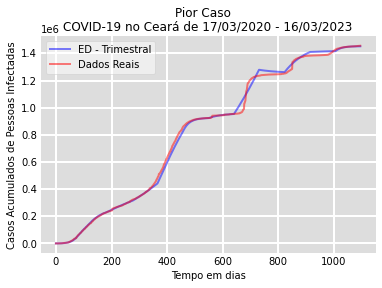
\includegraphics[width=3.5cm]{figuras/Exc24.png}}
        \caption{\label{fig:visualizapior}Sequência de Exclusão dos Métodos para o Modelo \ref{eq:ed2} no Pior Caso.}
    \end{figure}
\end{frame}

\begin{frame}{Resultados das Simulações Numéricas para o Ceará}
    \begin{figure}[ht]
        \center
        \subfigure[Busca Aleatória Global]{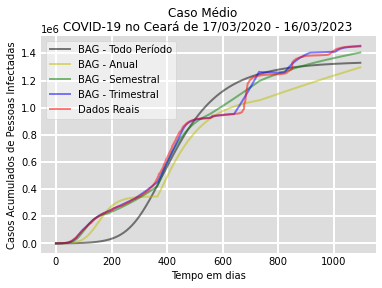
\includegraphics[width=3cm]{figuras/BAGCE3.png}}
        \qquad
        \subfigure[Busca Aleatória Local]{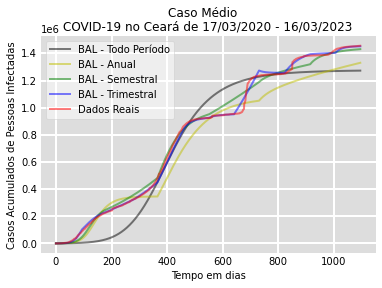
\includegraphics[width=3cm]{figuras/BALCE3.png}}
        \qquad
        \subfigure[Busca Harmônica]{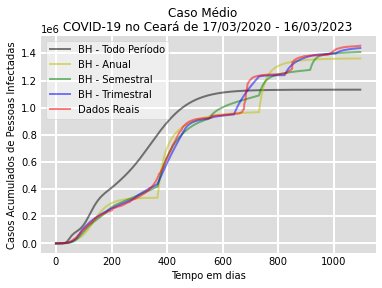
\includegraphics[width=3cm]{figuras/BHCE3.png}}
        \qquad
        \subfigure[Evolução Diferencial]{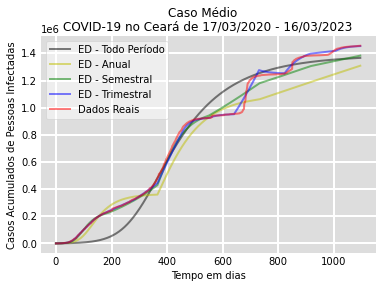
\includegraphics[width=3cm]{figuras/EDCE3.png}}
        \qquad
        \subfigure[\textit{Particle Swarm Optimization}]{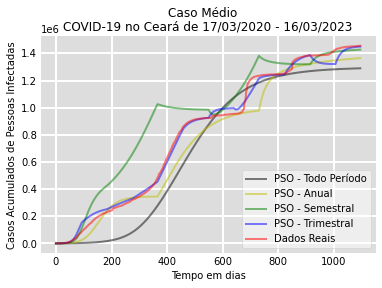
\includegraphics[width=3cm]{figuras/PSOCE3.png}}
        \caption{\label{fig:MetodosIsoladosMedioCasoCeara}Gráficos para o Modelo \ref{eq:ed2} no Caso Médio.}
    \end{figure}
\end{frame}

\begin{frame}{Resultados das Simulações Numéricas para o Ceará}
    \begin{figure}[ht]
        \center
        \subfigure[Todos os Métodos]{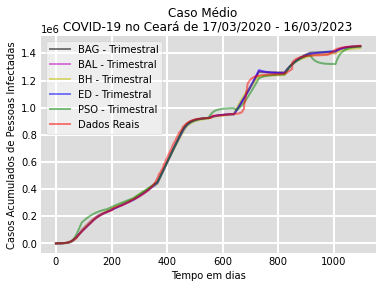
\includegraphics[width=4cm]{figuras/Exc17.png}}
        \qquad
        \subfigure[Exclusão do Método PSO]{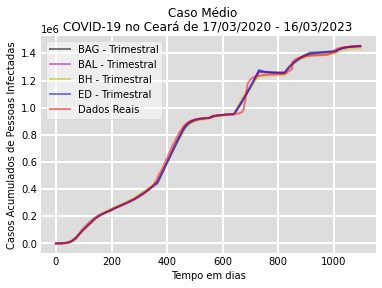
\includegraphics[width=4cm]{figuras/Exc18.png}}
        \caption{\label{fig:MetodosJuntosMedioCasoCeara}Sequência de Exclusão dos Métodos para o Modelo \ref{eq:ed2} no Caso Médio.}
    \end{figure}
\end{frame}

\begin{frame}{Período de Análise para o Brasil}
    \begin{table}[htbp]
        \centering
        \begin{tabular}{|c|c|c|c|}
            \hline
            Data Inicial & Data Final & Número de dias \\
            \hline
            26/02/2020   & 25/02/2023 & 1096           \\
            \hline
        \end{tabular}
        \caption{\label{tab:brto}Período de análise para o Brasil.}
    \end{table}

    \begin{table}[htbp]
        \centering
        \begin{tabular}{|c|c|c|c|}
            \hline
            Ano & Data Inicial & Data Final & Número de dias \\
            \hline
            1   & 26/02/2020   & 25/02/2021 & 366            \\
            \hline
            2   & 26/02/2021   & 25/02/2022 & 365            \\
            \hline
            3   & 26/02/2022   & 25/02/2023 & 365            \\
            \hline
        \end{tabular}
        \caption{\label{tab:bra}Partição anual do período completo para o Brasil.}
    \end{table}
\end{frame}

\begin{frame}{Período de Análise para o Brasil}
    \begin{table}[htbp]
        \centering
        \begin{tabular}{|c|c|c|c|}
            \hline
            Semestre & Data Inicial & Data Final & Número de dias \\
            \hline
            1        & 26/02/2020   & 25/08/2020 & 182            \\
            \hline
            2        & 26/08/2020   & 25/02/2021 & 184            \\
            \hline
            3        & 26/02/2021   & 25/08/2021 & 181            \\
            \hline
            4        & 26/08/2021   & 25/02/2022 & 184            \\
            \hline
            5        & 26/02/2022   & 25/08/2022 & 181            \\
            \hline
            6        & 26/08/2022   & 25/02/2023 & 184            \\
            \hline
        \end{tabular}
        \caption{\label{tab:brs}Partição semestral do período completo para o Brasil.}
    \end{table}
\end{frame}

\begin{frame}{Período de Análise para o Brasil}
    \begin{table}
        \centering
        \begin{tabular}{|c|c|c|c|}
            \hline
            Trimestre & Data Inicial & Data Final & Número de dias \\
            \hline
            1         & 26/02/2020   & 25/05/2020 & 90             \\
            \hline
            2         & 26/05/2020   & 25/08/2020 & 92             \\
            \hline
            3         & 26/08/2020   & 25/11/2020 & 92             \\
            \hline
            4         & 26/11/2020   & 25/02/2021 & 92             \\
            \hline
            5         & 26/02/2021   & 25/05/2021 & 89             \\
            \hline
            6         & 26/05/2021   & 25/08/2021 & 92             \\
            \hline
            7         & 26/08/2021   & 25/11/2021 & 92             \\
            \hline
            8         & 26/11/2021   & 25/02/2022 & 92             \\
            \hline
            9         & 26/02/2022   & 25/05/2022 & 89             \\
            \hline
            10        & 26/05/2022   & 25/08/2022 & 92             \\
            \hline
            11        & 26/08/2022   & 25/11/2022 & 92             \\
            \hline
            12        & 26/11/2022   & 25/02/2023 & 92             \\
            \hline
        \end{tabular}
        \caption{\label{tab:brtr}Partição trimestral do período completo para o Brasil.}
    \end{table}
\end{frame}

\begin{frame}{Resultados das Simulações Numéricas para o Brasil}
    \begin{figure}[ht]
        \center
        \subfigure[Busca Aleatória Global]{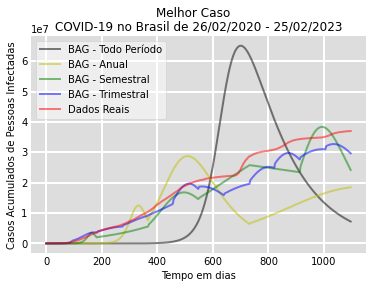
\includegraphics[width=3cm]{figuras/2BAGBR1.png}}
        \qquad
        \subfigure[Busca Aleatória Local]{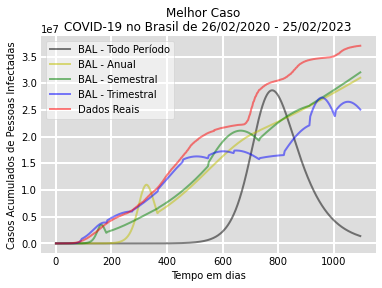
\includegraphics[width=3cm]{figuras/2BALBR1.png}}
        \qquad
        \subfigure[Busca Harmônica]{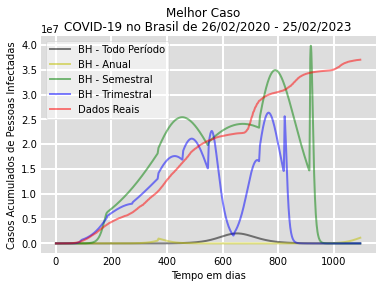
\includegraphics[width=3cm]{figuras/2BHBR1.png}}
        \qquad
        \subfigure[Evolução Diferencial]{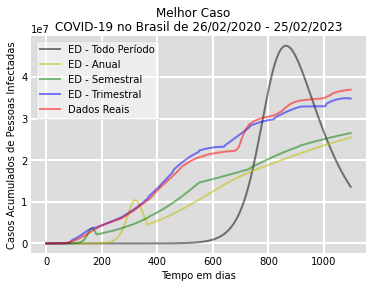
\includegraphics[width=3cm]{figuras/2EDBR1.png}}
        \qquad
        \subfigure[\textit{Particle Swarm Optimization}]{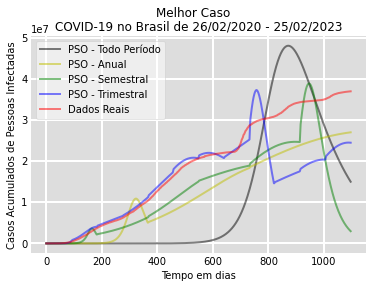
\includegraphics[width=3cm]{figuras/2PSOBR1.png}}
        \caption{\label{fig:MetodosIsoladosMelhorCasoModelo2Brasil}Simulações do Modelo \ref{eq:ed1} no Melhor Caso.}
    \end{figure}
\end{frame}

\begin{frame}{Resultados das Simulações Numéricas para o Brasil}
    \begin{figure}[ht]
        \center
        \subfigure[Busca Aleatória Global]{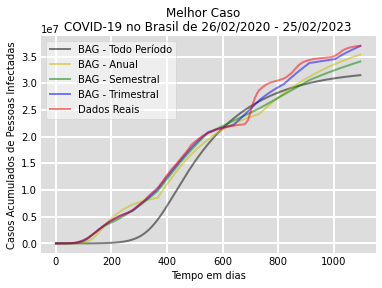
\includegraphics[width=3cm]{figuras/BAGBR1.png}}
        \qquad
        \subfigure[Busca Aleatória Local]{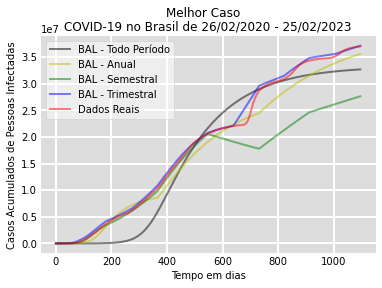
\includegraphics[width=3cm]{figuras/BALBR1.png}}
        \qquad
        \subfigure[Busca Harmônica]{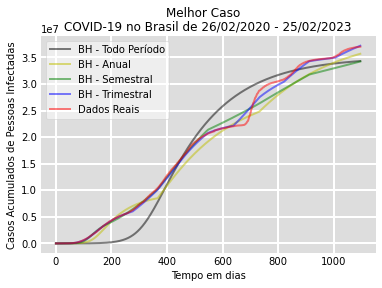
\includegraphics[width=3cm]{figuras/BHBR1.png}}
        \qquad
        \subfigure[Evolução Diferencial]{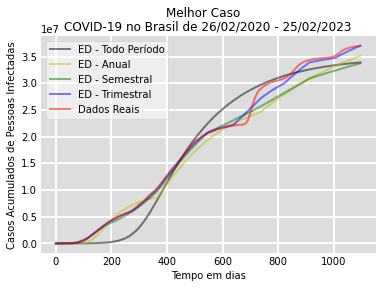
\includegraphics[width=3cm]{figuras/EDBR1.png}}
        \qquad
        \subfigure[\textit{Particle Swarm Optimization}]{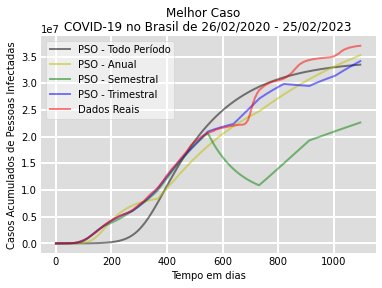
\includegraphics[width=3cm]{figuras/PSOBR1.png}}
        \caption{\label{fig:MetodosIsoladosMelhorCasoMModelo1Brasil}Simulações do Modelo \ref{eq:ed2} no Melhor Caso.}
    \end{figure}
\end{frame}

\begin{frame}{Resultados das Simulações Numéricas para o Brasil}
    \begin{figure}[ht]
        \center
        \subfigure[Modelo 1]{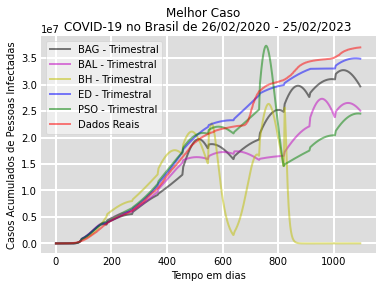
\includegraphics[width=5cm]{figuras/Exc11.png}}
        \qquad
        \subfigure[Modelo 2]{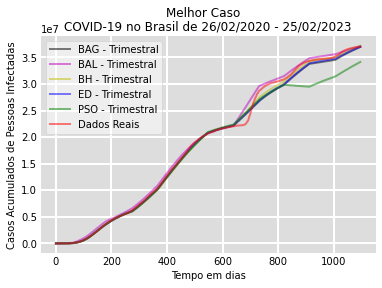
\includegraphics[width=5cm]{figuras/Exc10.png}}
        \caption{\label{fig:MetodosJuntosMelhorCasoBrasil}Comparação entre os Modelos 1 e 2 no Melhor Caso.}
    \end{figure}
\end{frame}

\begin{frame}{Resultados das Simulações Numéricas para o Brasil}
    \begin{figure}[ht]
        \center
        \subfigure[Todos os Métodos]{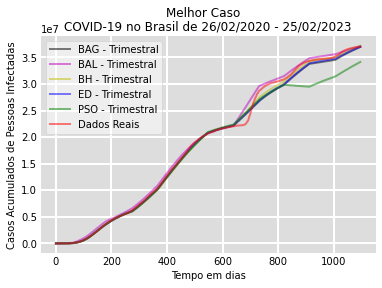
\includegraphics[width=3.5cm]{figuras/Exc13.png}}
        \qquad
        \subfigure[Exclusão do Método PSO]{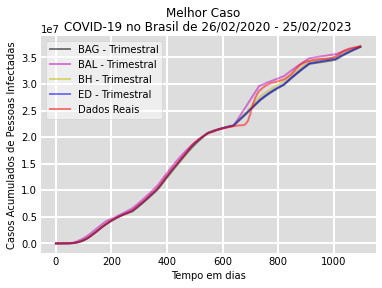
\includegraphics[width=3.5cm]{figuras/Exc14.png}}
        \qquad
        \subfigure[Exclusão do Método ED]{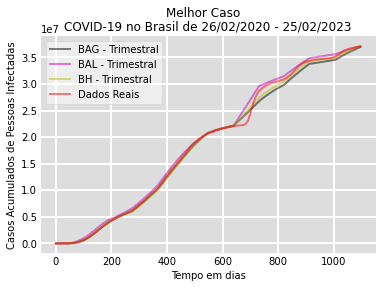
\includegraphics[width=3.5cm]{figuras/Exc15.png}}
        \qquad
        \subfigure[Exclusão do Método BAG]{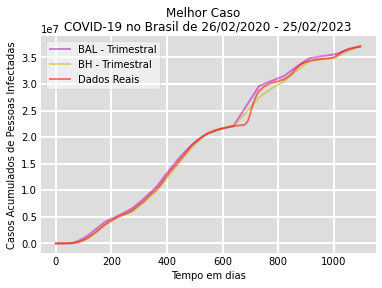
\includegraphics[width=3.5cm]{figuras/Exc16.png}}
        \caption{\label{fig:visualizaMelhorBrasil}Sequência de Exclusão dos Métodos para o Modelo \ref{eq:ed2} no Melhor Caso.}
    \end{figure}
\end{frame}

\begin{frame}{Resultados das Simulações Numéricas para o Brasil}
    \begin{figure}[ht]
        \center
        \subfigure[Busca Aleatória Global]{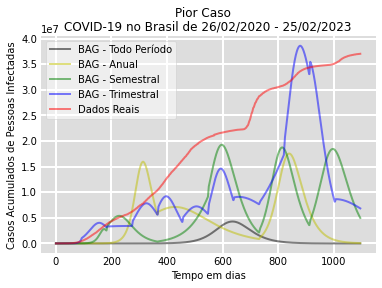
\includegraphics[width=3cm]{figuras/2BAGBR2.png}}
        \qquad
        \subfigure[Busca Aleatória Local]{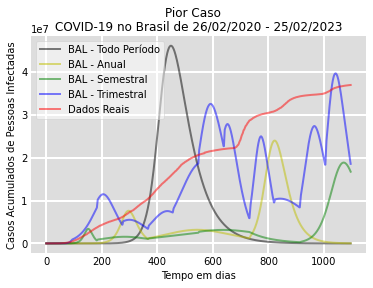
\includegraphics[width=3cm]{figuras/2BALBR2.png}}
        \qquad
        \subfigure[Busca Harmônics]{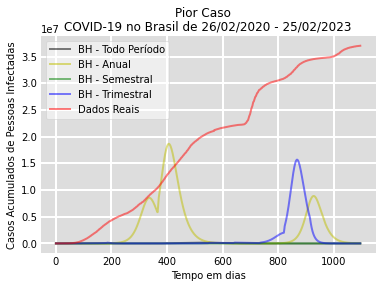
\includegraphics[width=3cm]{figuras/2BHBR2.png}}
        \qquad
        \subfigure[Evolução Diferencial]{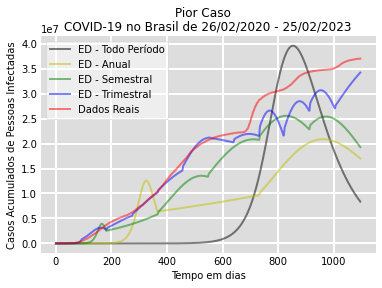
\includegraphics[width=3cm]{figuras/2EDBR2.png}}
        \qquad
        \subfigure[\textit{Particle Swarm Optimization}]{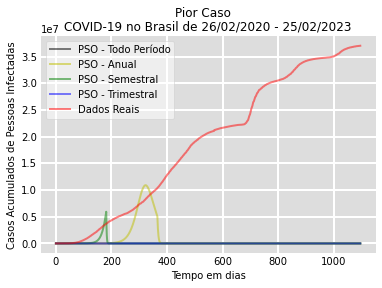
\includegraphics[width=3cm]{figuras/2PSOBR2.png}}
        \caption{\label{fig:MetodosIsoladosPiorCasoModelo2Brasil}Simulações do Modelo \ref{eq:ed1} no Pior Caso.}
    \end{figure}
\end{frame}


\begin{frame}{Resultados das Simulações Numéricas para o Brasil}
    \begin{figure}[ht]
        \center
        \subfigure[Busca Aleatória Global]{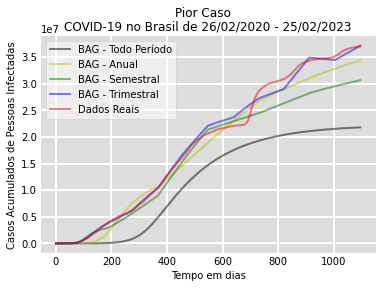
\includegraphics[width=3cm]{figuras/BAGBR2.png}}
        \qquad
        \subfigure[Busca Aleatória Local]{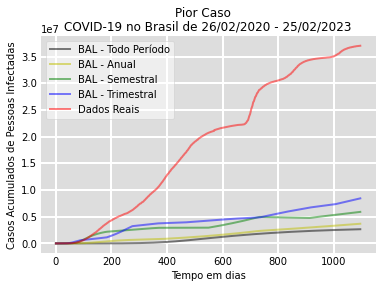
\includegraphics[width=3cm]{figuras/BALBR2.png}}
        \qquad
        \subfigure[Busca Harmônica]{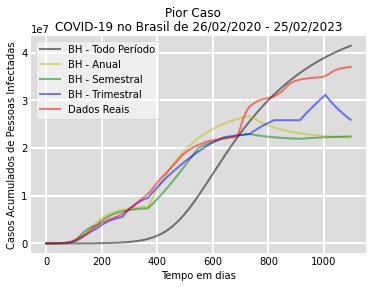
\includegraphics[width=3cm]{figuras/BHBR2.png}}
        \qquad
        \subfigure[Evolução Diferencial]{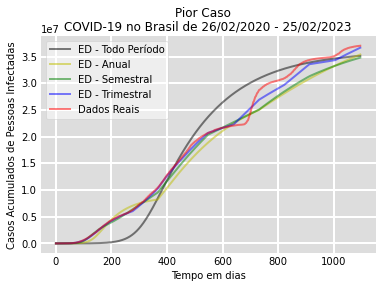
\includegraphics[width=3cm]{figuras/EDBR2.png}}
        \qquad
        \subfigure[\textit{Particle Swarm Optimization}]{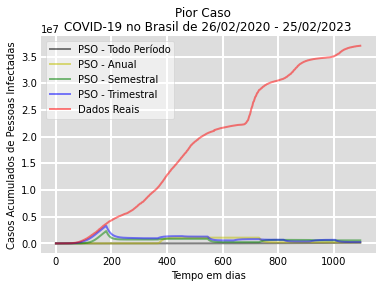
\includegraphics[width=3cm]{figuras/PSOBR2.png}}
        \caption{\label{fig:MetodosIsoladosPiorCasoModelo1Brasil}Simulações do Modelo \ref{eq:ed2} no Pior Caso.}
    \end{figure}
\end{frame}

\begin{frame}{Resultados das Simulações para o Brasil}
    \begin{figure}[ht]
        \center
        \subfigure[Modelo 1]{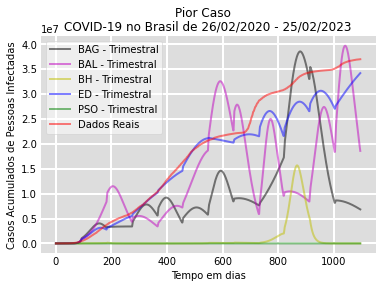
\includegraphics[width=4cm]{figuras/Exc12.png}}
        \qquad
        \subfigure[Modelo 2]{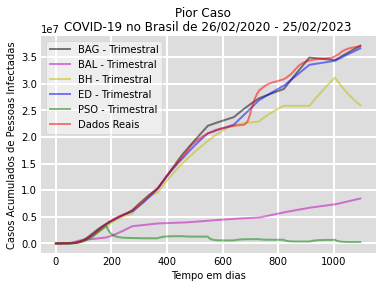
\includegraphics[width=4cm]{figuras/Exc5.png}}
        \caption{\label{fig:MetodosJuntosPiorCasoBrasil}Comparação entre os Modelos 1 e 2 no Pior Caso.}
    \end{figure}
\end{frame}

\begin{frame}{Resultados das Simulações Numéricas para o Brasil}
    \begin{figure}[ht]
        \center
        \subfigure[Todos os métodos]{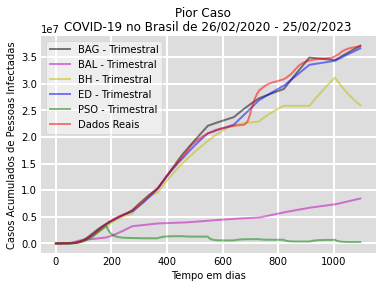
\includegraphics[width=3.5cm]{figuras/Exc5.png}}
        \qquad
        \subfigure[Exclusão do Método PSO]{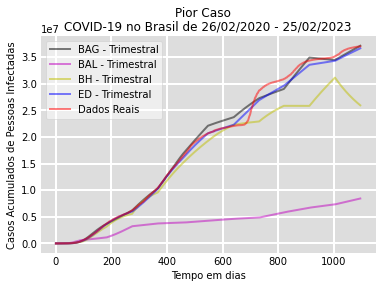
\includegraphics[width=3.5cm]{figuras/Exc6.png}}
        \qquad
        \subfigure[Exclusão do Método BAL]{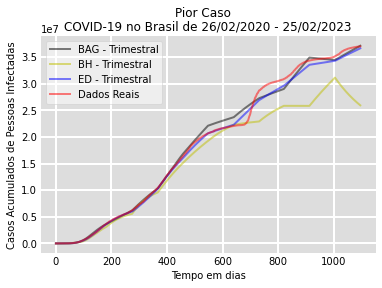
\includegraphics[width=3.5cm]{figuras/Exc7.png}}
        \qquad
        \subfigure[Exclusão do Método BH]{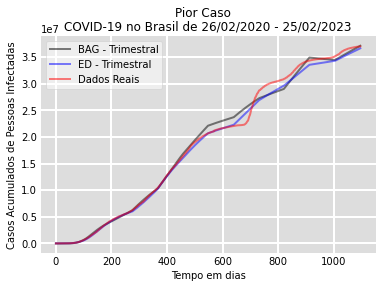
\includegraphics[width=3cm]{figuras/Exc8.png}}
        \caption{\label{fig:visualizapiorBrasil}Sequência de Exclusão dos Métodos para o Modelo \ref{eq:ed2} no Pior Caso.}
    \end{figure}
\end{frame}

\begin{frame}{Resultados das Simulações Numéricas para o Brasil}
    \begin{figure}[ht]
        \center
        \subfigure[Busca Aleatória Global]{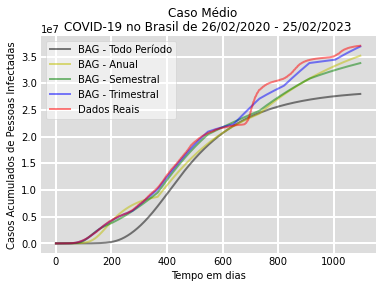
\includegraphics[width=3cm]{figuras/BAGBR3.png}}
        \qquad
        \subfigure[Busca Aleatória Local]{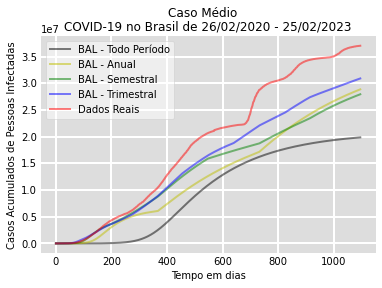
\includegraphics[width=3cm]{figuras/BALBR3.png}}
        \subfigure[Busca Harmônica]{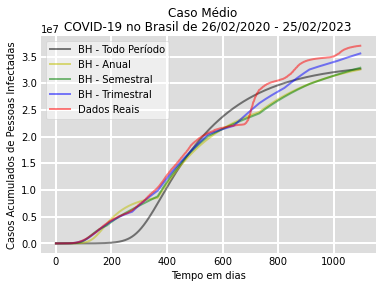
\includegraphics[width=3cm]{figuras/BHBR3 (2).png}}
        \qquad
        \subfigure[Evolução Diferencial]{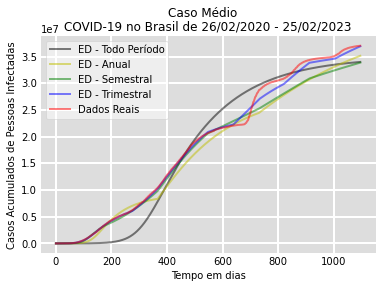
\includegraphics[width=3cm]{figuras/EDBR3.png}}
        \qquad
        \subfigure[\textit{Particle Swarm Optimization}]{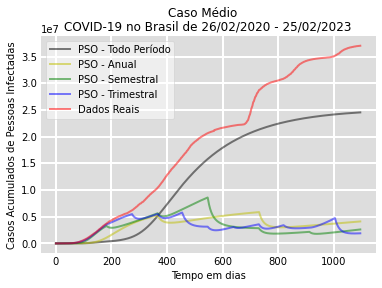
\includegraphics[width=3cm]{figuras/PSOBR3.png}}
        \caption{\label{fig:MetodosIsoladosMedioCasoBrasil}Simulações para o Modelo \ref{eq:ed2} no Caso Médio.}
    \end{figure}
\end{frame}

\begin{frame}{Resultados das Simulações Numéricas para o Brasil}
    \begin{figure}[ht]
        \center
        \subfigure[Todos os métodos]{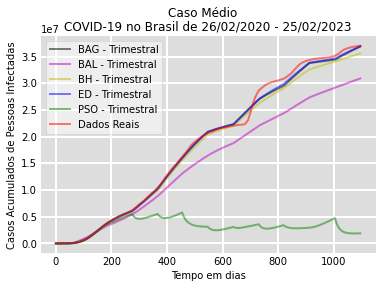
\includegraphics[width=3.5cm]{figuras/Exc1.png}}
        \qquad
        \subfigure[Exclusão do Método PSO]{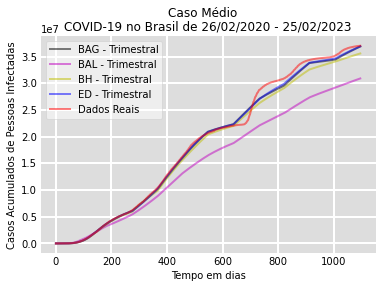
\includegraphics[width=3.5cm]{figuras/Exc2.png}}
        \qquad
        \subfigure[Exclusão do Método BAL]{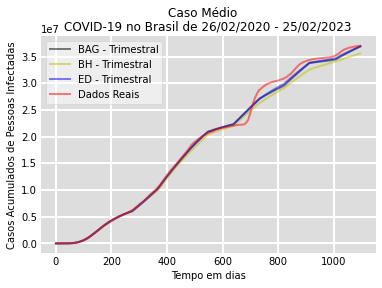
\includegraphics[width=3.5cm]{figuras/Exc3.png}}
        \qquad
        \subfigure[Exclusão do Método BH]{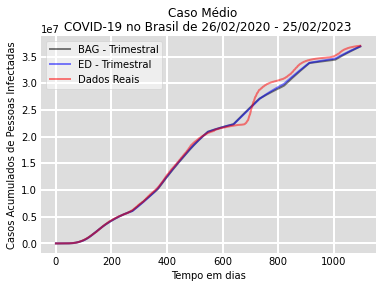
\includegraphics[width=3.5cm]{figuras/Exc4.png}}
        \qquad
        \caption{\label{fig:MetodosJuntosMedioCasoBrasil}Sequência de Exclusão dos Métodos para o Modelo \ref{eq:ed2} no Caso Médio.}
    \end{figure}
\end{frame}

\begin{frame}{Análise de Reprodutibilidade Basal para o Ceará}
    \begin{table}[htbp]
        \centering
        \begin{tabular}{|c|c|c|c|}
            \hline
            Trimestre & Data Inicial & Data Final & Valor de $\xi_0$            \\
            \hline
            1         & 17/03/2020   & 16/06/2020 & 2.5557587459895617          \\
            \hline
            2         & 17/06/2020   & 16/09/2020 & \textbf{1.4684688723918056} \\
            \hline
            3         & 17/09/2020   & 16/12/2020 & 1.4809625804599083          \\
            \hline
            4         & 17/12/2020   & 16/03/2021 & \textbf{3.8225473495081888} \\
            \hline
            5         & 17/03/2021   & 16/06/2021 & \textbf{1.6774136491962552} \\
            \hline
            6         & 17/06/2021   & 16/09/2021 & \textbf{5.8019805524507255} \\
            \hline
            7         & 17/09/2021   & 16/12/2021 & \textbf{1.9937798120787482} \\
            \hline
            8         & 17/12/2021   & 16/03/2022 & \textbf{4.1751349557200506} \\
            \hline
            9         & 17/03/2022   & 16/06/2022 & 2.593026182245002           \\
            \hline
            10        & 17/06/2022   & 16/09/2022 & 2.5235528038881645          \\
            \hline
            11        & 17/09/2022   & 16/12/2022 & 1.1914799269420324          \\
            \hline
            12        & 17/12/2022   & 16/03/2023 & 2.5041004240181115          \\
            \hline
        \end{tabular}
        \caption{\label{tab:repce}Valor do parâmetro $\xi_0$ em cada trimestre no Ceará \cite{povo2023}}
    \end{table}
\end{frame}


\begin{frame}{Análise de Reprodutibilidade Basal para o Ceará}
    \begin{table}[htbp]
        \centering
        \begin{tabular}{|c|c|c|c|}
            \hline
            Trimestres & Diferença de $\xi_0$          \\
            \hline
            1 e 2      & -1.0872898735977561           \\
            \hline
            2 e 3      & \textbf{0.0124937080681027}   \\
            \hline
            3 e 4      & 2.3415847690482805            \\
            \hline
            4 e 5      & -2.1451337003119336           \\
            \hline
            5 e 6      & 4.1245669032544703            \\
            \hline
            6 e 7      & -3.8082007403719773           \\
            \hline
            7 e 8      & 2.1813551436413024            \\
            \hline
            8 e 9      & -1.5821087734750486           \\
            \hline
            9 e 10     & \textbf{-0.06947337835683752} \\
            \hline
            10 e 11    & -1.3320728769461321           \\
            \hline
            11 e 12    & 1.3126204970760791            \\
            \hline
        \end{tabular}
        \caption{\label{tab:difce}Diferença entre o valor de $\xi_0$ no trimestre atual e o valor no trimestre anterior no Ceará}
    \end{table}
\end{frame}

\begin{frame}{Análise de Reprodutibilidade Basal para o Brasil}
    \begin{table}[htbp]
        \centering
        \begin{tabular}{|c|c|c|c|}
            \hline
            Trimestre & Data Inicial & Data Final & Valor de $\xi_0$           \\
            \hline
            1         & 26/02/2020   & 25/05/2020 & 3.5157594269143093         \\
            \hline
            2         & 26/05/2020   & 25/08/2020 & \textbf{5.505172675815306} \\
            \hline
            3         & 26/08/2020   & 25/11/2020 & 6.534072188874569          \\
            \hline
            4         & 26/11/2020   & 25/02/2021 & 4.861051197766502          \\
            \hline
            5         & 26/02/2021   & 25/05/2021 & 6.265221444710935          \\
            \hline
            6         & 26/05/2021   & 25/08/2021 & \textbf{6.989886588032348} \\
            \hline
            7         & 26/08/2021   & 25/11/2021 & \textbf{6.508067883553517} \\
            \hline
            8         & 26/11/2021   & 25/02/2022 & 4.717985649671903          \\
            \hline
            9         & 26/02/2022   & 25/05/2022 & 6.746780435011656          \\
            \hline
            10        & 26/05/2022   & 25/08/2022 & 5.341040873547087          \\
            \hline
            11        & 26/08/2022   & 25/11/2022 & 6.241582399947055          \\
            \hline
            12        & 26/11/2022   & 25/02/2023 & 5.706965216405303          \\
            \hline
        \end{tabular}
        \caption{\label{tab:repbr}Valor do parâmetro $\xi_0$ em cada trimestre no Brasil \cite{fiocruz2023}}
    \end{table}
\end{frame}

\begin{frame}{Análise de Reprodutibilidade Basal para o Brasil}
    \begin{table}[htbp]
        \centering
        \begin{tabular}{|c|c|c|c|}
            \hline
            Trimestres & Diferença de $\xi_0$        \\
            \hline
            1 e 2      & 1.989413248901              \\
            \hline
            2 e 3      & 1.028899513059263           \\
            \hline
            3 e 4      & -1.673020991108067.         \\
            \hline
            4 e 5      & 1.404170246944433           \\
            \hline
            5 e 6      & 0.724665143321413           \\
            \hline
            6 e 7      & -0.481818704478831          \\
            \hline
            7 e 8      & \textbf{-1.790082233881614} \\
            \hline
            8 e 9      & \textbf{2.028794785339753}  \\
            \hline
            9 e 10     & -1.405739561464569          \\
            \hline
            10 e 11    & 0.900541526399968           \\
            \hline
            11 e 12    & -0.534617183541752          \\
            \hline
        \end{tabular}
        \caption{\label{tab:difbr}Diferença entre o valor de $\xi_0$ no trimestre atual e o valor no trimestre anterior no Brasil}
    \end{table}
\end{frame}

\section{Conclusões e Trabalhos Futuros}
\begin{frame}{Conclusões}
    \begin{itemize}
        \item O Modelo SIR se revelou uma ferramenta de grande valor para a avaliação do número acumulado de casos de COVID-19;
        \item Entre os dois modelos do tipo SIR utilizados neste estudo, o modelo \ref{eq:ed2} demonstrou ser o mais apropriado para ajustar-se aos dados observados nas duas regiões analisadas
        \item Entre os métodos de Inteligência Computacional empregados na estimação dos parâmetros dos modelos \ref{eq:ed1} e \ref{eq:ed2}, o método ED destacou-se ao obter o conjunto mais preciso de parâmetros estimados, sobretudo na região do Ceará
        \item Entre as partições do período completo utilizadas para aprimorar o desempenho do método de Inteligência Computacional aplicado ao sistema epidemiológico, a subdivisão mais eficaz foi a partição trimestral.
    \end{itemize}
\end{frame}

\begin{frame}{Trabalhos Futuros}
    \begin{itemize}
        \item A abordagem intervalar e a abordagem \textit{fuzzy} serão empregadas com o objetivo de compreender as incertezas no comportamento dinâmico da COVID-19 nas duas regiões abordadas neste trabalho.
        \item As redes neurais artificiais serão aplicados ao sistema epidemiológico para estimar os parâmetros, com o propósito de realizar uma comparação com os métodos de Inteligência Computacional utilizados neste estudo.
        \item Os métodos de aprendizado de máquina serão usados para analisar os dados da COVID-19.
    \end{itemize}
\end{frame}

\begin{frame}[allowframebreaks]{Referências}
    \fontsize{5}{10}\selectfont
    \bibliography{demo}
\end{frame}

\begin{frame}{Agradecimentos}
    \begin{center}
        Obrigado pela atenção!!!
    \end{center}
\end{frame}

\end{document}



